\section*{Project Description}

\iflater\todo{Remember to not use any URLs in the project description!
  (They are encouraged in the references.)}\fi

Testing plays a vital role in modern software development processes,
contributing crucially to robustness and overall quality---as well as
to overall development costs.
%
It comes in many styles---unit testing, integration testing,
performance testing, stress testing, accessibility testing,
etc.---supported by many sorts of tools, with yet more advanced tools
and techniques continually being developed, studied, and applied.

One such technique, {\em property-based testing} (PBT), has been
enthusiastically taken up by the functional programming research
community, since its introduction in the QuickCheck
library~\cite{ClaessenHughes00} in Haskell, and is beginning to make
serious inroads beyond academia.
%
PBT is sometimes explained as ``formal specification without formal
verification''---a developer characterizes a the desired behavior of
some piece of code at a high level, in the form of executable {\em
  properties}, which are simply Boolean-valued functions; the code is
then validated against these properties by running it over and over
with a large number of automatically generated test cases.
%
PBT tools thus give programmers an efficient way of testing their
software's behavior with a comprehensiveness that is often not
possible with alternative tools.

PBT's combination of rich, high-level specification with easy, mostly
automatic validation has proved effective at identifying subtle
bugs in telecommunications software~\cite{arts2006testing}, replicated
file~\cite{hughes2014mysteries} and key-value
stores~\cite{Bornholt2021}, automotive software~\cite{arts2015testing}, and a range
of other real-world systems~\cite{hughes2016experiences}. With support
now available in all major programming languages, PBT has
begun to make significant inroads in the broader software
industry---for example, the developers of the Hypothesis library for
Python estimate that it has on the order of half a million
users~\cite{ZacPersonalCommunication}.

\newcommand{\participant}[1]{{P#1}}
% \newcommand{\participant}[1]{{\bf P#1}}

After all these successes, one might wonder if the research community has already
addressed all of the challenges that could limit PBT's adoption
in the broader software industry, but it
seems the answer is no.
In an ongoing need-finding study with users of OCaml's QuickCheck testing tool
at Jane Street Capital, we found
consistent enthusiasm for PBT---participants called it it
``obviously valuable'' [Participant \participant{1}],
built their own libraries for it when standard ones were not available in their
development context [\participant{8},
\participant{21}], and suggested that ``everyone'' at the company should use it
[\participant{20}]. But we also found
challenging new research questions based on developer concerns.
Specifically, the developers we have spoken with so far
%
(a) sometimes struggle
to identify all the situations where properties are readily accessible for
testing,
%
(b) they complain that it
can be difficult to write random generators for data structures
with complex invariants or to tune generator distributions to
adequately explore the space of interesting test cases,
%
(c) they find
it hard to understand whether their properties and generators are
effectively testing their software, and
%
(d) they are disappointed by
the paucity of educational and training materials for introducing
newcomers to PBT.\iflater\bcp{All that needs final tuning.}\fi

Solutions to these challenges will demand insights from both the
programming languages (PL) and
human-computer interaction (HCI) communities.  Chasins et
al.~\cite{chasins_pl_2021} argue that PL+HCI is a ``sweet spot'' that marries
``need-finding techniques [to] identify ...  programmers' current and future
pain points'' with tools that ``help [programmers] write safe and correct
programs.'' We wholeheartedly agree.
The team behind this proposal is uniquely positioned to advance the state of
PL+HCI: PI Head is deeply embedded in the HCI community and recently co-founded
the new HCI group of the University of Pennsylvania, while PI Pierce is has
published in every corner of the PL world and has decades of experience in both
researching and teaching about programming languages. This proposal will be the
first of many PL+HCI projects that the University of Pennsylvania Computing and
Information Science department undertakes.\iflater\hg{I'm just spitballing,
feel free to change}\fi

We propose a comprehensive, interdisciplinary research program that
will bring the combined power of PL and HCI approaches to bear,
accelerating PBT's transition into practice\iflater\bcp{do we need
  this?} and creating a blueprint for further research\fi.
\begin{itemize}[noitemsep]
  \item
  Our ongoing study (described in more detail below) is
  just the first step in our formative research.
  We will further explore the challenges PBT faces in
  industry by conducting three additional
  studies---two survey studies and one observation study of
  PBT users {\em in situ} (\sectionref{sec:foundation}).
  \item We will address challenges in property specification by developing a
  conceptual framework of high-impact PBT use cases, along with tools that
  enhance PBT in common use-cases like model-based testing and extend that set
  of use cases with the ability to write properties over logged output
  (\sectionref{sec:spec}).
  \item We will address challenges in test-case generation with new
  domain-specific languages for expressing generators that enable novel
  algorithms for PBT tasks like generation of precondition-satisfying values,
  test input mutation, and example-based generator tuning.
  (\sectionref{sec:gen}).
  \item We will address gaps in validation of testing effectiveness by providing
  users with powerful new ways of interacting with their generators and test
  suites that give them visibility into the bug-finding power of their tests
  (\sectionref{sec:val}).
  \item We will create comprehensive educational resources for training developers and
  university students in best practices for PBT (\sectionref{sec:ed}).
\end{itemize}
We conclude the proposal with a concrete outline of our work plan
(\sectionref{sec:plan-of-work}) and discussion of the broader impacts of the
proposed work (\sectionref{sec:broader-impacts})

\iflater\bcp{This needs a bit of focusing and toning down at some point.}\fi
The projects we undertake will be motivated by
foundational need-finding research in the software industry, including, but not
limited to, the aforementioned study with Jane Street. Some projects will have a
clear PL flavor, focusing on domain-specific languages and type-based tools that
will make PBT tools more powerful and flexible; but we will motivate and
evaluate them with techniques from HCI. Other projects will focus on the HCI elements
of PBT, building better interfaces and experiences for developers; yet their
implementation will draw from our wealth of PL knowledge. In this way, we craft
a holistic research agenda around PBT that is sure to be both well motivated and
well founded.

\sectionstar{Orientation: Property-Based Testing}
Before discussing our motivating study, we briefly explain what PBT is
and why it is important.

Popularized by QuickCheck~\cite{hughes2007quickcheck} in Haskell,
PBT is a form of random testing~\cite{hamlet1994random} where
users write executable functions, usually in the same language as
their System Under Test, which act as partial
specifications of a function under test. For example, a user might
write the following property of the \lstinline{insert}
function for an implementation of a binary search tree (BST):
\begin{lstlisting}
  prop_insertCorrect x t  =  (isBST t ==> isBST (insert x t))
\end{lstlisting}
This property takes only a single
line to express, yet it can be used to validate a limitless number of
input-output pairs. Concretely, it is
a simple function that takes two arguments and returns a
Boolean value: true if the property is satisfied, and false if it is
not. The function \texttt{prop\_insertCorrect} checks
that an insert operation on a binary search tree preserves the
binary ordering of the tree; it states
that, given an arbitrary tree \texttt{t} and an integer
\texttt{x} to insert into that tree, if the original tree
satisfies the
binary search tree invariant (``\texttt{isBST t}''), then it should remain
a BST following the insertion of \texttt{x} (``\texttt{isBST (insert x t)})''.

Given a property like this one, the PBT tool chooses large number of inputs and
checks that the property evaluates to \lstinline{True} for each input; any input
that causes the property to fail is reported as a {\em counterexample}.  This
proposal is on property-based {\em random} testing~\cite{hamlet1994random}, in
which these inputs are chosen randomly.
There are other approaches, including enumerative test-case
generation~\cite[etc.]{DBLP:conf/haskell/RuncimanNL08, leancheck} and model
checking, but random generation remains the dominant approach in the PBT
space. Its surprising effectiveness is often attributed to the
``combinatorial'' nature of larger test cases: bugs can often be
exposed by test inputs with a specific combination of features,
independent of whatever other features may be present---for example,
by any sequence of API calls that includes calls to four particular
functions in a particular order, even if these calls happens to be
interleaved with other API calls.  This means that testing with one
big structure has the effect of testing with exponentially many
smaller sub-structures. Both practical experience and theoretical
arguments~\cite{goldstein2021dojudgeatest} suggest that this effect is quite
powerful---i.e., we can discover small counterexamples by generating
a few larger test inputs containing combinatorially many diverse
sub-structures rather than systematically enumerating test inputs
beginning with the smallest ones.

From the perspective of a user, applying PBT happens in a series of steps:
(1) Define one or more properties that should be true of the program under
  test.
(2) Design (or otherwise obtain) {\em random input generators} for the
  values that the properties take as input.
(3) Check the properties with generated inputs, using infrastructure
  provided by the PBT framework.
And (4) if counter-examples are found, make sense of them and determine the
  source of the bug.
Each of these steps presents opportunities to improve the user experience of
PBT, as we shall see below.

\smallskip

Why go to the trouble of PBT, when more straightforward example testing is the
de-facto standard in the software industry? First and foremost, PBT has the
potential to be much more thorough than user-defined examples. As mentioned
previously, PBT has an impressive track-record uncovering bugs that other
approaches to testing had failed to find~\cite{arts2006testing,
hughes2014mysteries, Bornholt2021, arts2015testing, hughes2016experiences}. But
PBT is more than just thorough---it is actually more general than example-based
testing. Wrenn et al.~\cite{wrenn2021using} point out that example-based testing
of programs like that implement relations (e.g., topological sort, which may
produce one of a number of potentially correct results) is impossible to do
faithfully; a property-based specification is a much better choice. PBT is also
obviously preferable if formal properties already exist; this is the use-case
for QuickChick~\cite{paraskevopoulou_foundational_2015}, which implements PBT in
the Coq proof assistant. Finally, PBT can act as superior documentation:
participants in our foundational study (\participant{5}, \participant{21})
talked at length about properties being an ideal way to communicate what a
program is supposed to do.

With so many potential advantages, it is clear that PBT should be a tool that
software developers have readily at their fingertips. We plan to put it there.

\iflater\todo{Double-check that we've mentioned all relevant
  ``hgih-level'' related work somewhere.}
  \hg{My current decision is that Orientation should stay high-level RE PBT.
  Specifically, I think it shouldn't get into the weeds of generation
  techniques, including fuzzing. I added a bunch of references RE that later on
  in the context sections.}
  \fi

\sectionstar{Motivation: A Formative Study of PBT in Industry \pagebudget{2}}\label{sec:motivation}
%
The technical goals of this proposal are grounded in early
findings from an ongoing need-finding study asking {\em How can the
  research community make PBT more valuable for software developers?}
%
\iflater \todo{Sentence to justify why
we did the study}\bcp{If needed...}\fi
%
% \subsectionstar{Study Population}
%
In this study, we have conducted semistructured interviews with
PBT stakeholders at Jane
Street Capital---both
developers who have had exposure to PBT as
well as developers of PBT tools.

Interview
studies are a common tool for early-stage need finding in
HCI research, yielding highly informative stories about people, the tasks they need to
accomplish, and the tools they use to accomplish them. The goal
is to identify a broad set of opportunities for improving PBT tools,
grounded in concrete, detailed, authentic stories from developers.

Jane Street is among of the world's largest
financial market-makers; its 1700 employees
include around 700 software developers.  A number of features make
it an attractive setting for this study.  Most importantly, PBT is
already well established at Jane Street, so there is a large
population of people with well-informed opinions on its benefits and
challenges.  Also, Jane Street famously builds almost all of its
software in OCaml, a mostly functional programming language with
strong support for rich static typing and modularity, plus a well-engineered
PBT tool. This unified
ecosystem allows us to control for a number of potentially confounding
factors: all of the developers have access to the same tools,
libraries, language-level programming abstractions, house coding
rules, social conventions, etc.

\iflater
\bcp{Not sure we need to say all (or any) of this, but maybe?  If we
  keep it, we'll need a bit of transition to the next paragraph.}%
\proposecut{Ideally, the study population would have included both
users
and {\em non}-users of PBT. In reality, it is difficult to recruit and
have meaningful conversations with non-users of a technology. Our
strategy, instead, was
to recruit across as broad a spectrum of usage as could be reasonably found
at our partner institution, including both frequent users of PBT technologies,
as well as a handful of
developers who had had only limited, occasional exposure to PBT. Our
proposed survey
study (\sectionref{sec:survey}) aims to establish contact with a broader
sample of non-users of PBT to assess opportunities for making PBT tools more
valuable and discoverable for this group.}
\hg{I think I'm in favor of cutting. I do like the idea of a forward pointer to
  the survey, but we sort of already do that in the next paragraph}
\bcp{Let's take one more look at it in a few days before deleting for
  good...}
\fi

There is a danger that findings from a study at a single firm with a homogeneous
OCaml-based testing ecosystem may not generalize outside of this
ecosystem. Part of our proposed work is to carry out further user
studies targeting a broader and more diverse community
(\sectionref{sec:foundation}).  However, Jane Street itself is quite
diverse in the sorts of software it builds, including real-time
trading, quantitative algorithms, networked systems, and hardware
description code~\cite{signalsandthreads}, and our study participants
come with a wide variety of experiences and requirements.

Our interview instrument---the script used to loosely
structure the interviews---and our analysis process were developed and
tested through a prototype study with seven users of the Hypothesis
PBT toolkit, recruited over Twitter.  This analysis yielded a
conceptual framework of barriers to usage of PBT, which we published
recently at the SPLASH HATRA workshop, one of the key venues for
emerging work on human aspects of formal methods tools and type
systems~\cite{goldstein2022some}.

At the time of writing, the full
complement of 30 interviews and a preliminary round of analysis have
been completed; full-scale analysis will begin in 2023.

\subsectionstar{Organizing Themes} The main theoretical output from
this qualitative study will be a collection of {\em Themes} summarizing
and categorizing our observations about the ways Jane Street developers
use PBT, what they need from it, and how the research community be
able to help.  While deep analysis of the interview transcripts remains
to be done, several themes are already apparent in our real-time
notes, and these form the backbone of the present proposal.

\newcommand{\proptheme}[1]{{\color{nord-orange} \em #1}}
\newcommand{\gentheme}[1]{{\color{nord-green} \em #1}}
\newcommand{\evaltheme}[1]{{\color{nord-purple} \em #1}}
A first set of
themes revolves around the {\bf specifications} that developers test.
% and the kinds of programs in which they choose to test them.
Since
PBT is often described as a kind of lightweight formal method, one
might imagine that a central challenge would be coming up with the
right specifications. Indeed, an earlier pilot study of PBT users in
Python~\cite{goldstein_problems_2022} that we ran to prepare for the Jane Street
study\iflater\bcp{Is this the first
  mention of the pilot study?  If not, move this citation earlier and
no need for it here.}\fi{}
concluded just that.
  But at Jane Street itself
we actually heard very little about difficulties coming up with
properties; rather, most participants described applying PBT in
\proptheme{High-Leverage Scenarios} where properties were already
available or straightforward to invent.  For example, \participant{9} pointed out
that PBT is particularly easy to apply when one has ``a really good abstraction
with a complicated implementation.''
Several participants (\participant{3}, \participant{15},
\participant{20}, \participant{22}), when asked to speculate, guessed
that 80--100\% of Jane Street
developers write programs like this, where properties are easy to find, and
where PBT is relatively easy to apply.  This suggests that an effective way to
approach education and documentation around PBT would be to focus on
``opportunistic'' applications of PBT as an easy on-ramp.

Our interviews also identified several \proptheme{Opportunities for Better
Leverage}---situations where PBT is not easy {\em yet}, but could be with a
little more research effort. For example, \participant{7} spoke about trying to
test a poorly abstracted program (which are notoriously resistant to PBT) by
writing properties about output it prints to the terminal; we plan to
operationalize this approach.
Furthermore, more than three quarters of study participants had used a
particular kind of PBT, commonly called
\proptheme{Model-Based Testing}.
\participant{3}, an author of PBT tools at Jane Street, considered better
automation and tooling around model-based testing to be one of the most
significant ways improve PBT and make it easier to pick up and use.

We discuss plans for work that addresses \proptheme{specification
  themes} in \sectionref{sec:spec}.

\smallskip

Another set of common themes in the interviews concerned the {\bf generation} of
random inputs for property-based testing. Many participants spoke
highly of the \gentheme{Derived Generators} that can be inferred from
the OCaml type system (\participant{5} called OCaml's tools for this
``[expletive] amazing'' and \participant{30} called them a ``game changer'').
These generators are already quite good, but they could be better: participants
identified deficiencies both small (e.g., API quirks) and large (e.g.,
derived generators
cannot enforce semantic preconditions). When derived generators
failed, participants fell back to \gentheme{Bespoke Generators}, which
are far more flexible but proportionally more time consuming to design and work
with. For example, \participant{20} found important bugs with a bespoke
generator for XML documents,
but reported spending ``at least a day'' writing it.
Improving the abstractions available for writing bespoke generators would
greatly improve both the experience of using PBT and its potential for
bug-finding.

If a generated input is deemed a {\em counter-example} for a property,
highlighting a bug in the code, it needs to be easy to use that input to
determine the root cause of the bug. The interviews made clear that
\gentheme{Shrinking}, the process of finding the smallest possible input that
provokes a given bug, is a critical part of the PBT process.  \participant{8}
and \participant{21}, who each needed to implement their own PBT libraries, both
made sure to include shrinkers in their implementations. Unfortunately, getting
shrinking right, especially for values that must satisfy preconditions, is
difficult.

We discuss plans for work that addresses \gentheme{generation themes} in \sectionref{sec:gen}.

\smallskip

A final category of common themes concerned the {\bf validation} of testing
effectiveness. As with any sort of testing, when doing PBT it is difficult to
know when ``enough is enough.'' One standard approach is to simply test up to a
time limit, but participants' approaches to \evaltheme{Budgeting Time for PBT}
were anything but standardized.
Most of our interviewees run PBT testing just for a few seconds per property,
expecting that the bulk of the necessary testing is done in hundreds or up to
around a thousand examples, but some run it for much longer.
Interestingly, the opposite was true about a close cousin of PBT, fuzz testing.
Participants \participant{14} and \participant{20}, who used both PBT and
fuzzing tools, ran the fuzzers for far longer
% HG: Don't change this from "year" to "CPU-year" -- he really ran AFL for A YEAR
(\participant{14} ran the fuzzer for over a year!).

It would be easier for developers to make informed decisions about
time budgets for testing if
they had better access to feedback about how well their testing is doing.
Indeed, \evaltheme{Evaluation of Effectiveness} often featured in our
conversations.
There are many forms such feedback could take, from code coverage (requested by
\participant{9} and \participant{25}) to input space coverage measurements
(requested by \participant{10}, \participant{16}, and \participant{16}) and even
strategies like {\em mutation
  testing}~\cite{papadakis_mutation_2018}.

We discuss plans for work that addresses
\evaltheme{validation themes} in \sectionref{sec:val}.
\amh{I feel like this section does not yet make a convincing
case that the current practices around validation are
problematic.}

\iflater
\amh{Let's foreshadow other findings that
we will publish that are outside of the scope of this proposal, but which might
be motivating to other researchers, including: developers could benefit from
additional automated support for deriving generators from types, effectiveness
budget (i.e., deciding how much time to spend on running PBT tests versus fuzz
tests), integration with unit testing frameworks, and exploring the use of
properties as a source of documentation.}
\bcp{Not sure where is the right place for this discussion (or if
  there will be space)...}
\fi

% \todo{Debugging doesn't really fit here...}
\ifdesperateforspace
\bcp{ We could save a tiny bit of space by grouping all the
  ``We discuss'' sentences into a paragraph at the end.  But if space
  is OK, I think it reads well this way.}
  \fi

\SECTION{Foundation}{Understanding Needs and Opportunities \pagebudget{1}}{sec:foundation}

% \amh{This section is around double its page budget. One reason is that I am
% probably being too heavy-handed in trying to justify the methodological choices.
% Help me figure out what to prune!}\bcp{Did some pruning! :-)}

The final results from the in-progress user study should paint a clear
picture of the benefits and challenges of PBT in the specific context
of Jane Street and other organizations with similar characteristics.  But to
fully understand the potential impact of PBT across the software
industry---and the factors that may limit its adoption---we need to
cast a wider net.
%
In this section, we describe three planned studies, drawing on mixed
methods in the service of producing a comprehensive and actionable
agenda for future research, in this research project and beyond---two
written surveys, one to assess the generality of these needs and obstacles
and one to identify potential for adoption of PBT tools
(\sectionref{sec:survey}), and an observation study to understand
particular tasks involved in PBT to guide the design of new algorithms
and interactive tools (\sectionref{sec:observations}).

\iflater\bcp{Somewhere, we need to mention the letter of support from
  JS.  I guess it belongs in the section where we describe potential
  further collaborations with them.}\fi

\SUBSECTION{Generalizing the Findings from Jane Street}{sec:survey}{1}{1}
\iflater\bcp{Plural or singular?}\fi

Our ongoing Jane Street study has already revealed a number of
opportunities to improve tools for property-based testing. To identify
others, and to better understand which of these opportunities are most
important for the research community to explore, we will conduct two
surveys, each with a broad sample of developers. These surveys aim to
(1) determine which obstacles observed in the interview study
represent widely experienced pain points with PBT tools and
(2) characterize the potential benefits of better tools to the
software industry as a whole.

\emph{Validation survey}. Our interview study has revealed
a number of issues with existing PBT tools, but it is not clear
how broadly these issues are experienced by developers, or
their relative severity. To find out, we will conduct a survey
asking developers which of the issues we have identified are
ones they have experienced, and the severity of those issues
in their experience. Respondents will also be asked to report on
other issues that have arised in their use of PBT tools.
To provide
clear usage scenarios to guide future work, respondents will
be asked to write brief anecdotes elaborating on the
most severe issues they encountered.

Respondents will
be recruited broadly, from three sources. First, we will recruit
users of Hypothesis, a widely used Python-based PBT
framework
% \footnote{In personal communications, one of the
% maintainers of Hypothesis estimates that Hypothesis has
% approximately 500k current users. \amh{I am not sure if we
% should include this. It sounds too big to be true to
% me.}}
% BCP: Already mentioned at the top
(see the attached letter of support).
Second, we will distribute the survey at Jane Street, hoping to reach
a broader set of developers than we were able to interview.
And third, we will recruit users from social media by posting
survey announcements from the PIs' Twitter and Mastadon
accounts, tagging the functional programming and testing
communities.
\amh{Do we have any connections that would give
us access to functional programming or testing-related
software development conferences?}
\bcp{Sure. What would we do with them?}
Types and types-announce mailing lists. They are mailing
lists for the types programming. We will distribute announcements among
attendees of conferences like ICFP or ``Yow!'' whom have
a cumulative thousands of programmers with functional
programming experience.

\emph{Impact survey}. Is PBT the sort of
technology that could one day be used by every developer? To get a
sense of this, we survey ``proximal'' users of PBT---that is,
developers who do not use PBT currently, but who experience
use cases where PBT methods would be particularly useful,
once designed to fit their tasks and workflows. Particular
attention will be given to those whose work requires the
writing of validation code and public APIs with some
definition of types. We will recruit a broad sample of
participants across development contexts (professional, open
source, educational) by working with our industry contacts
and by recruiting over social media. \amh{I am not sure this
survey feels quite right. It feels really hard to conduct in
a way that we get a convincing answer to our question of
``who would use PBT if the tools were sufficiently
well-designed?''}\bcp{Indeed---feels weaker than the other.}
\hg{Yeah, I think the question is important, but I don't know we really know how
to anwer it at this stage. One option is to piggy-back on the When to Specify
It! work, and ask ``how many of these situations do you encounter once every X
months at your job.'' That doesn't find the upper bound we want, but it'd find a
much better lower bound.}

\SUBSECTION{An Observation Study of PBT in Practice}{sec:observations}{2}{2}

Anecdotes related in interviews do not generally, in and of
themselves, provide enough information to inform the design of
effective tools---they beg questions like: (1) How much time
are participants willing to devote to
a task like creating a generator or debugging a counterexample when in the
middle of a programming task? (2) How much space is available on a developer's
screen (amidst other tools like code editors and terminals) for
interacting with new
tools? (3) What are developers' current strategies for solving the
problems they describe
(for example, what representations of generated data currently seem most helpful
for programmers trying to under the distributions of data generated by a
generator)?.  As a basis for designing tools with a substantial novel interface
component (see \sectionref{sec:val}), we will observe developers
undertaking the respective PBT tasks we
aim to support, on the order of a small handful of developers (i.e., 2--10
observation sessions). These observation sessions will allow us to evolve
singular anecdotes from the interviews into a more comprehensive picture of
what kinds of designs will be viable for helping programmers.

% \bcp{Again, we need to explain the expected contributions---what end
%   does ``characterizing obstacles'' serve.}

\smallskip

Together, the studies described in this section provide a firm foundation many
of the activities in this proposal, and for future research on PBT more
generally. We will produce a validated and prioritized set of developer needs
for PBT tools and a detailed set of requirements for how tools should be
(re)designed to best satisfy the most important of those needs.

\SECTION{Specification}{Widening the On-Ramp \pagebudget{2}}{sec:spec}
The projects in this section address the \proptheme{specification themes}
discussed in the Motivation section. In \sectionref{sec:whento}, we discuss a
plan to aggregate and communicate a comprehensive list of PBT patterns that
developers can use to decide if PBT is an easy choice for testing their code.
Then in \sectionref{sec:outpurprop} we describe a plan to significantly expand
that list of patterns, and in \sectionref{sec:automating} we focus in on a
particular pattern and provide tools to apply it automatically. Together, these
projects will greatly improve the on-ramp to PBT and clarify its place in the
software industry.

\SUBSECTION{Properties Over Logs}{sec:outpurprop}{2}{3}

One common problem raised by Jane Street developers (and even more loudly
in our earlier pilot study~\cite{goldstein2022some}) was
that code may sometimes not be abstracted
in a way that is amenable to testing. Indeed, any kind of
testing of software units---with PBT techniques or otherwise---requires
``units'' to test!  But PBT is
especially sensitive to issues like poorly encapsulated global state, which may
impact the repeatability of testing, and leaky or confusing
abstraction boundaries, which make it difficult to cleanly state
properties or specifications.

One Jane Street developer (\participant{7}) described their experience testing
a trading system (we'll call it System A) with messy abstraction boundaries. In
this case, System A was hard to test because it was primarily used as a
sub-component of a larger System B: System B would take in simple data, and then
at some point pass a large, complex data structure to System A, which would do
some work and hand results back to System B. PBT of System A was therefore hard,
because generating valid examples of the large data structure that System A
takes as input required deep knowledge of the internals and types of System B
that the developers of System A did not have access to, and because the
interface was too complex to write straightforward properties about.

One might imagine trying to test System A through System B by writing properties
over intermediate values in System A. One might imagine trying to write and
test properties like
\begin{lstlisting}
  sublist_of processed (next (processed))      (* 1. Processing is monotonic. *)
  msg.length < 100 ==> never (overflow = true) (* 2. Capacity at least 100 bytes. *)
  eventually (processed.length = msg.length)   (* 3. The whole message is processed. *)
\end{lstlisting}
which demonstrate that internal variables like \lstinline{processed},
\lstinline{msg}, and \lstinline{overflow} evolve correctly over time.
These properties could theoretically be tested without ever running System A on
its own: we can generate inputs to System B, have System B drive System A, and
simply monitor the variable values to check the desired properties.

The tricky part comes with how to actually implement this testing. One might
hope to do it through debug assertions, but that quickly becomes untenable.
Checking the property (1) with debug assertions would require noisy code to
saves the previous value every time \lstinline{processed} is updated, and the
programmer would need to use macros or some other kind of meta-programming to
remove that code when building in release mode. Even worse, there may be no way
to check properties (2) or (3) at all! Doing so would require making an
assertion at the ``end'' of the computation, which may not actually be possible
if System B is driving System A from the outside.

Instead, we propose a framework for writing properties over {\em logged values}
that can capture the interesting relationships between past and future variable
values that the above properties demand.  Concretely, we will insert lightweight
logging annotations and provide a language for writing properties over those
logs. In order to express concepts like \lstinline{next}, \lstinline{never}, and
\lstinline{eventually} the property language will need some logical connectives
that are not standard in PBT.  In particular, we need a temporal logic like {\em
linear temporal logic} (LTL) so that properties can capture a notion of time.

Using LTL with PBT is not unheard of---Quickstrom testing
framework~\cite{oconnor_quickstrom_2022} has already shown that LTL properties
can be used for specifying and testing graphical user interfaces---but LTL
properties at this level of generality have not yet been attempted. We plan to
compile the user's LTL formulae to properties over traces that respect the
structure of the log and ignore updates to irrelevant variables. Then, the
developer can provide inputs to some system containing the sub-system under
test, and the test harness will apply the trace properties in real time. In this
way, the user can get feedback about the invariants that should hold of the
intermediate values of their programs, making PBT available in a huge range of
programs where it was previously too difficult to apply.

\SUBSECTION{Automating Model-Based PBT}{sec:automating}{2}{3}
\hg{Talked to Richard: he suggested a few variations on this theme that are also
interesting.
\begin{itemize}[noitemsep]
  \item One ``parent'' signature with two diverging ``children'': figure out how
  to test implementations of the children against each other
  \item What if the signatures aren't the same, but they're isomorphic? He's
  testing the unboxed float module against the boxed float module; those sigs
  are different (types aren't equal) but they are isomorphic...
\end{itemize}
I didn't get a chance to talk to Joe, but hopefully between these ideas and some
more stewing we can find the right angle}

One finding that has surprised us from the Jane Street study
is that it is {\em very} common for developers to
build (or already to have) a {\em model implementation} of the code
they are testing and
check that the two versions of the code agree on randomly generated
sequences of API calls.
This is a well-documented approach to PBT~\cite{hughes_experiences_2016}, but it
is not supported as well as it could be by existing tooling. For example,
interviewees described setting up {\em very similar}
model-based PBT harnesses for at least three different projects. Each harness
is specific to the problem at hand, so the hard work of setting up these tests
has no hope of being reused from one project to another, but the logic behind
the harnesses is ripe for automation.

The APIs that the Jane Street developers tested came in the form of ML-style
{\em modules}. The module systems of OCaml and other
ML-based languages are theoretically interesting and extremely expressive, and
they are objects of study in their own right~\cite{macqueen_modules_1984}. We propose
new, type-based automation for model-based testing of these kinds of modules,
building both theoretical and practical tools for understanding the ways that
their APIs can be exercised.

We will work from first-principles, building a model of ML-module {\em traces}.
This model will need to capture the various initial inputs that need to be
generated, the output values that should be checked for agreement, and, most
importantly, all of the ways that outputs from one call can flow to inputs of
another. Since these values are all typed, this model will likely need to be
dependently typed to maintain all necessary invariants.

Concretely, the tools we build will take a model signature, for example
\begin{lstlisting}[language=Caml]
  module Map : sig
    type ('k, 'v) t
    val get : ('k, 'v) t -> 'k -> 'v option
    val put : ('k, 'v) t -> 'k -> 'v -> ('k, 'v) t
  end
\end{lstlisting}
and generate a series of calls like
\begin{lstlisting}[language=Caml]
  let m = put m 1 2; get m 1; let m = put m 1 3; m get 1
\end{lstlisting}
that manipulate the data structure and query its contents.
\bcp{Prior work on testing polymorphic code seems relevant here---citations!}
When testing two
different implementations of \lstinline{Map}, the developer can verify that the
two implementations produce the same results for each of the operations in the
sequence. The automated tooling could also insert checks for internal
invariants, ensure that one operation executes at least as quickly as another,
and insert other checks that are simple to specify but tedious to implement
manually.

With the prevalence of ML-derived languages used in practice today, and with ML
modules' similarities to other tools for defining interfaces, this project has
the potential to significantly increase the usability of model-based
PBT.

\bcp{Not very convincing.  For one thing, we neither make a case that
  solving this problem for ML modules will generalize (at all, much
  less straightforwardly) to other languages with different modularity
  mechanisms.  At the same time, we don't convey they technical
  challenge of doing it even for ML.}
\hg{Same problem as the previous section---I'm working from hunches here. Maybe
we should take a half hour to talk through these projects?}
\bcp{Definitely.}

\SECTION{Generation}{Better Tools for Random Inputs \pagebudget{3}}{sec:gen}
%
The Jane Street study also highlighted several \gentheme{generation themes}.
Generators were regularly cited
as one of the most challenging parts of the
PBT process, and many
asked for better tools for constructing generators that reliably address
their testing goals. In this section, we describe a series of projects
to develop new and better ways to express random data generators that give
developers more automatic ways to test their code more thoroughly.

\subsectionstar{Context: Why is Random Generation Hard?}%
As discussed in the Orientation, PBT relies heavily on {\em random data
generators}. The inputs produced by the generator exercise the developer's
properties and give confidence that they hold---provided the inputs are
interesting enough.

{\em Preconditions.}
Many properties that developers want to test have {\em preconditions}
(or {\em validity conditions} or {\em input constraints}) that
restrict the set of inputs that should be used for testing. This comes up often
when testing data structures with invariants that must hold in order to apply
the operations under test. Testing such properties can be problematic, because
many preconditions are difficult to satisfy randomly; if the developer is not
careful their testing may waste most of its time budget generating and
discarding invalid inputs.

{\em Coverage of Realistic Inputs.}
Worse, even among valid inputs, not all are equally realistic. Often generated inputs
feel fabricated, since they are not constructed with prior knowledge of the
kinds of inputs that the program is likely to see.

{\em Distributional Concerns.}
Worse yet, even with validity and realism accounted for, there are other ways for
generators to under-perform. In particular, the spaces of inputs that generators
target is often very large, and the best generators explore as much of the space
as possible, as quickly as possible.

The PBT literature partially addresses these concerns, with solutions solving
one problem at the expense of another and trading off between programmer effort
and generator power.
The existing solutions
fall on a spectrum from automatic to manual. The automatic approaches use
proxies for validity and general ``interestingness'' of inputs: some, like {\em
fuzzers}~\cite{afl-readme}, optimize readily available metrics like code
coverage, others ask users to provide metrics~\cite{loscher2017targetedpbt}, and
naturally some use machine learning to infer proxies for
validity~\cite{godefroid2017learn, DBLP:conf/icse/ReddyLPS20}. These approaches
are easy to apply and can obtain good distribution coverage, but they are rarely
sufficient for testing properties with complex preconditions. Slightly more
manual approaches are based on declarative representations of validity
conditions: for preconditions that are primarily structural, {\em grammar-based
fuzzing} provides a compelling solution~\cite{godefroid2008grammar,
holler2012fuzzing, veggalam2016ifuzzer, wang2019superion,
srivastava2021gramatron}, and for more complex, semantic preconditions, some
have proposed using SMT-solvers~\cite{dewey2017automated, LuckPOPL,
steinhofel2022input} to automatically seek out valid inputs. These tools are
much better at satisfying up to moderately-complex properties, but some are
still out of reach. The semi-automatic
category also includes tools for {\em example-based tuning}, a process that
improves realism of inputs by mimicking user-provided
examples~\cite{soremekun2020inputs}; the existing tools successfully generate
more realistic inputs, but are again limited in the preconditions they can
satisfy.

\subsectionstar{Context: Monadic Generators}
\iflater\hg{Not sure I love this transition... I liked it better when this sentence was above}\fi
The most manual, but also the most flexible, solutions use hand-written
generators, written in a convenient domain-specific language (DSL).
In  Haskell, where PBT was
first popularized, many such DSLs are implemented using {\em
monads\/}~\cite{moggi1991notions}, an elegant design pattern for
expressing effectful (in this case, random and stateful) computations
in a pure, stateless underlying
language. While monadic DSLs are not actually necessary to express generators in
non-pure languages, some libraries (e.g., in OCaml) still use monadic
abstractions to build their generator DSLs.

Monadic generators can implement random data producers of arbitrary complexity
(e.g., it is possible to write a monadic generator for Haskell
programs~\cite{palka_testing_2011}), so they are often more expressive than
other representations like grammar-based generators.  Yet monadic generators are
syntactically constrained in a way that isolates the probabilistic code and
prevents usage errors (like passing the wrong random seed around). As we will
see, the constrained nature of monadic generators also makes them the perfect
candidates for sophisticated manipulations and interesting generalizations.

\subsectionstar{Context: Free Generators}
In order to improve monadic generation along the dimensions listed
above, it helps to re-frame generators as {\em parsers of randomness}. A generator
operates by making a series of random choices, but we can equivalently think of
it as being provided some random sequence of choices and then simply following
those choices to produce a value. This perspective has been used in a few
implementations of PBT
systems~\cite{maciver2019hypothesis, dolan2017testing}; we made it
formal in our paper, {\em Parsing Randomness}~\cite{goldstein2022parsing}.

The paper introduces {\em free generators}, which generalize the standard
monadic generator abstraction, demonstrate a formal link between parsing and
random generation, and enable new algorithms for generation that improve
generation modulo validity constraints. Free generators are written the same
way as standard monadic generators, but they are more like generator ``plans''
or syntax trees.%
\footnote{For experts: Free generators are implemented using {\em freer
monads}~\cite{kiselyov2015freer}, which have been used to great effect in recent
years to capture the structure of effectful computations
(cf.~ITrees~\cite{old:xia2019interaction}). Freer monads represent
monadic computations syntactically by reifying the monad operations
(\lstinline{return} and \lstinline{>>=}) as data constructors. Critically, this
is all implemented within the language (no macros or AST
manipulation). See \cite{goldstein2022parsing} for more details on the
free generator representation.}
This means that a single free generator can be be {\em interpreted} in multiple
different ways. In {\em Parsing Randomness} we prove that any free generator can
be interpreted either as a standard monadic generator or as a source of
random choice strings with a parser over those strings; this formalizes the
relationship between generators and parsers. Furthermore, since free generators
are uninterpreted syntax trees, they can be manipulated programmatically. Free
generators admit a version of a Brzozowski
derivative~\cite{brzozowski1964derivatives} that can be used incrementalize
generation. We showed that free generator derivatives enable an algorithm called
{\em Choice Gradient Sampling}, which uses repeated derivatives to guide a
generator to inputs that are more likely to be valid with respect to a given
precondition. This work is an important step towards better automation for
generators with complex preconditions.

\SUBSECTION{Reflective Generators}{sec:reflective}{1}{2}
\bcp{Maybe this is also better described as proposed work?}\hg{Could be, but I
worry that enough of the following projects rest on reflective generators that
we want to be able to say ``don't worry, we actually have an idea what these
will look like''}\bcp{That's fair enough.  I think we can finesse this
issue though---e.g., by mentioning that we've been discussing this
with Sam and Meng and have some concrete ideas how to proceed (and
then giving a bit of technical meat, though of course there is not
room for much).}
\hg{Fine by me. How do you want to frame the reference to Sam and Meng?}
Continuing on from the free generator work, we have begun to look at even more
powerful generalizations of the standard monadic approach to random generation.
One such project concerns monadic generators
that can be run {\em backward}.

If a generator parses a sequence of choices into a value, then running the
generator backward should take a value and produce a sequence of choices that
would produce that value. With this in mind, we propose {\em reflective
generators}, an extension of monadic generators that can be run backward to
``reflect'' on the choices that they made when producing an input. The machinery
that makes reflective generators work is quite complex,%
\footnote{Reflective generators are both monads and {\em
    partial profunctors},
implementing bidirectional programming in the style of Xia et
al.~\cite{xia2019composing}. This approach to bidirectional programming is
related to lenses~\cite{foster2009bidirectional}, but it hides much of the
complexity of bidirectional program composition in the bind operation of the
monad. The result is an elegant programming experience where both directions of
the computation can be written at once, in a type-safe way.}
but, like free generators, their syntax is still quite close to that of normal
monadic generators.

But reflective generators are useful for more than just generation!
We plan to explore (at least) the following two example applications.

{\em Validity-Preserving Mutation.} Many automated testing algorithms
(especially fuzzing algorithms~\cite{afl-readme}) {\em mutate} values to explore
the behavior of the program in a space ``around'' those values. This can be
difficult in PBT scenarios, where values are subject to complex validity
constraints, since mutation often produces invalid values. Reflective
generators can help: we can (1) reflect on the choices that lead to a particular
value, (2) mutate those choices, and (3) re-run the generator with the new
choices {\em while correcting any choices that
would lead to an invalid value.} Figure~\ref{fig:mutation} shows the way this
algorithm is able to mutate a binary search tree, while maintaining validity,
using no BST-specific code beyond the reflective generator itself.

\begin{figure}[h]
  \centering
  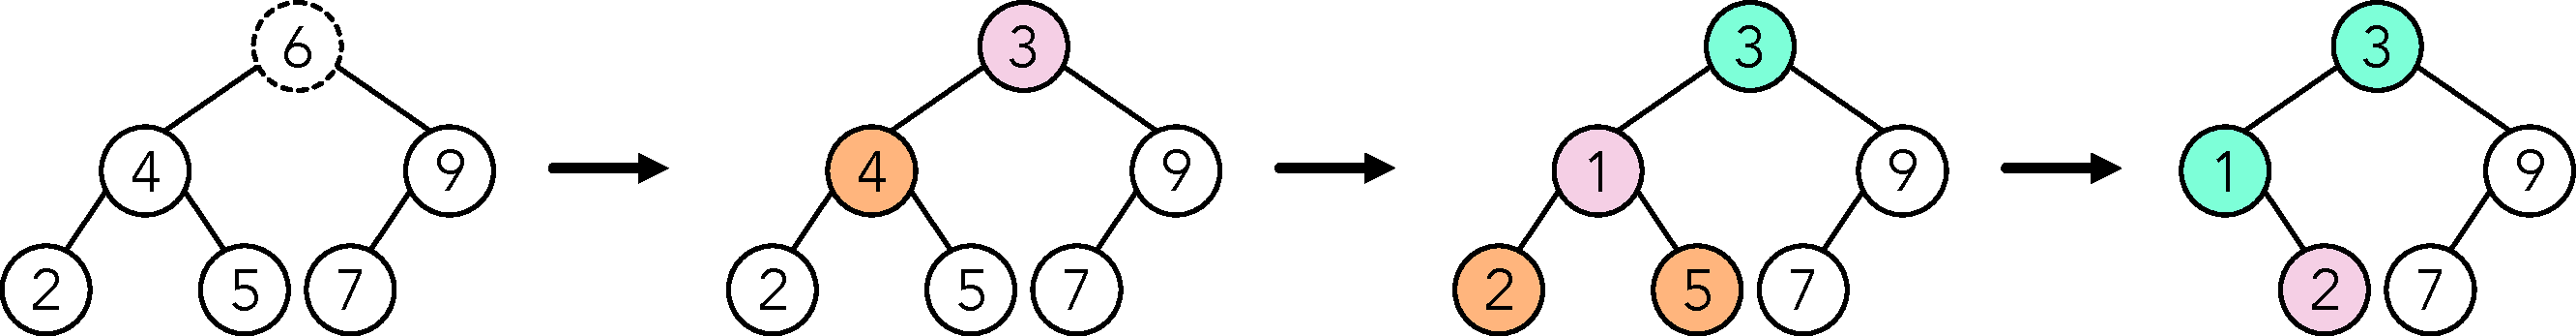
\includegraphics[width=.6\textwidth]{assets/mutate-diagram.pdf}
  \caption{Validity-preserving mutation of a binary search tree, maintaining the
  BST invariant.}\label{fig:mutation}
\end{figure}

{\em Example-Based Tuning.} Earlier we pointed out that good generators
produce ``realistic'' inputs; one way to ensure this is to tune the generator so
it produces values that are similar to some user-supplied values deemed
realistic. Existing tools make good use of this example-based approach to
tuning~\cite{soremekun2020inputs}, but they do not work with generators as
powerful as monadic generators. We implement a similar algorithm using
reflective generators: we can (1) again, reflect on the choices that lead to a
set of realistic values, and (2) run the generator with {\em new choice weights}
informed by the choices that we saw.

Both of these applications have the potential to significantly improve
testing effectiveness---example-based tuning helps users generate more
realistic inputs, while validity-preserving mutation enables more
automated approaches to improving generator distributions---and we get
{\em both} by upgrading our existing generators to reflective ones. We
will see some additional use cases for reflective generators in the
following sections.

\SUBSECTION{Bringing Fuzzing into Focus}{sec:fuzzing}{2}{3}
{\em Fuzzers} like AFL~\cite{afl-readme} use principles that are similar to the
ones behind PBT: they leverage randomized testing to quickly exercise as
many program behaviors as possible.  One might then expect that the fuzzing and
PBT share a significant amount of literature, but in reality they do not. Often
the communities seem to ``talk past'' one another.

We propose that the main thing separating the PBT and fuzzing communities is
simply a difference of {\em focus}. The fuzzing literature mostly talks about
fast and automatic ways to find critical (security) vulnerabilities in
programs---usually manifesting in the form of crash failures.  In contrast, PBT
researchers want effective ways to test semi-formal logical specifications of
their programs. Both areas of focus are important: fuzzing captures the ``80\%''
of cases catching high-profile bugs with minimal programmer effort, and PBT
gives a level of thoroughness that fuzzing does not claim to match. But there is
something unsatisfying when things are laid out this way. In particular, while
fuzzing and PBT focus on different testing problems, they face many of the same
technological hurdles. Both PBT and fuzzing need fast and effective ways to
generate random inputs that are valid for the systems that they are testing, and
neither community has truly settled on the ``right'' way to get there.

There is already some work that attempts to bridge the gap between PBT and
fuzzing. For example, the FuzzChick library in Coq~\cite{OLDlampropoulos19fuzzchick}
uses code coverage as guidance for PBT and the HypoFuzz library uses a
similar approach in Python~\cite{hatfield-dodds_hypofuzz_nodate}. These projects
are demonstrably powerful, but neither benefits from the years of expertise
poured into industrial-strength fuzzers; Crowbar
does~\cite{dolan2017testing}. Crowbar uses
AFL~\cite{afl-readme}, one of the best-established
fuzzers, to generate random bit-strings that are later parsed into program
inputs.  (We plan to use AFL++~\cite{fioraldi_afl_2020},
which has supplanted the original AFL project.)

\begin{wrapfigure}{l}{0.5\textwidth}
  \centering
  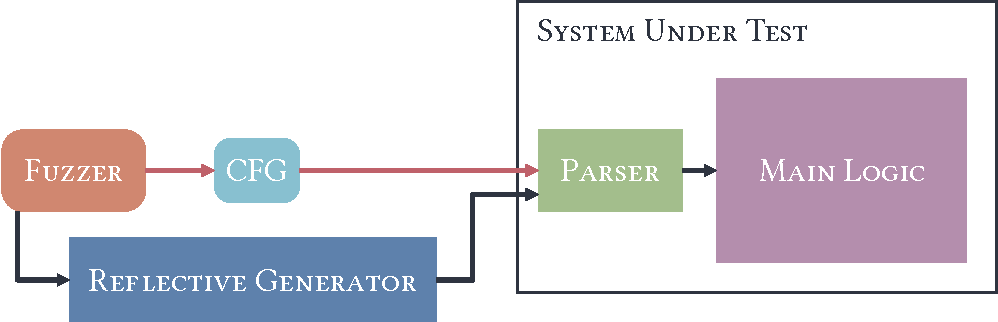
\includegraphics[width=.4\textwidth]{assets/fuzzing.pdf}
  \caption{Overview of gradually constrained fuzzing.}\label{fig:fuzzing-plan}
\end{wrapfigure}

Our system will start with a setup similar to Crowbar, but with a much greater
focus on the generators; in particular, we will use reflective generators to
gain significant testing power. The setup is shown in
Figure~\sectionref{fig:fuzzing-plan}. We start with a classic fuzzing setup, attempting
to make the system under test crash by passing it a variety of semi-random
inputs. Normally, the fuzzer is working against the parser, in the sense that
the parser's job is to reject invalid inputs and the fuzzer's job is to ``get
past the parser.'' The CFGs used by grammar-based fuzzers help a bit, but they
cannot generate inputs satisfying complex context-sensitive constraints. As in
Crowbar, we avoid this adversarial relationship and subsume grammar-based
generation with a powerful generator that is powerful enough to satisfy the
parser by construction; in our case, that generator is reflective.

Why use a reflective generator? First, we should clarify why any kind of monadic
generator is preferable to grammar-based options. Monadic generators can
straightforwardly generate context-free structures, and they can often do so
automatically with the help of type information~\cite{mista2019deriving}. If
this is all that the precondition requires, then there is no harm in using a
monadic generator, rather than a grammar-based one. But the beauty of a monadic
generator is that it can be made far more powerful, incrementally, as the
developer's testing needs change. The developer can start off thinking that they
need only consider the structure of their inputs, but they can later add more
semantic guarantees if they determine that their testing is ineffective.

Focusing on reflective generators specifically, one compelling benefit is that
their backward interpretation can be used to help seed the fuzzer.  Most fuzzers
ask for a number of {\em seeds}, input examples that the fuzzer can start from,
in order to ensure that the fuzzer does not spend ages exploring
inputs that have no hope of working out. Normally these seeds are easy enough
for the user to write down, since they are simply program inputs, but now that
we are asking the fuzzer to generate sequences of choices it becomes much more
error-prone (and tedious) to produce seeds by hand.  This is one great use for a
backward interpretation. The user can write down their seeds---either as values
in the program, or as text that can be parsed by the program's parser---and then
the reflective generator can reflect on the choices that produce those seeds.

The reflective generator also provides validity-preserving mutation. Guided by
heuristics, the system can opt to supplement the fuzzer's mutation schedule with
mutations that are obtained by the reflective generator's validity-preserving
mutation (which is more targeted than the mutators provided by the fuzzer). We
expect this to have a significant impact on performance, especially in contexts
where preconditions are relatively sparse and therefore hard for AFL++ to mutate
correctly.

Our ultimate goal is a grand unification of PBT and fuzzing generator tooling:
the fuzzing literature provides battle-tested heuristics for coverage-guided
generation, the PBT literature provides powerful tools like reflective
generators for refining generator performance incrementally, and both
communities benefit from generators with better distributions.

\SUBSECTION{Reflective Shrinking}{sec:shrinking}{3}{4}
\bcp{Could we swap this with the previous section?  Would make the
  wprk plan (progression of section titles) look a bit tidier...}

A more modest application of reflective generators uses them to implement
validity-preserving {\em shrinking} of values to find smaller counterexamples
and speed up debugging. On its face, this feels similar to validity-preserving
mutation: Can we reflect on choices, shrink the choices, and then re-run the
generator with the smaller choices? Likely yes! But there are complications.
When mutating, it is often fine if the mutated value is accidentally quite
different from the original value, since the mutator is trying many values and
any that catch a bug are equally good. But when shrinking, it is often very
important to get another input that is both smaller and, ideally, provokes the
{\em same bug}. These nice properties are likely within reach, but care will
need to be taken to ensure that shrinkers behave as expected.

\SUBSECTION{Empirically Evaluating PBT Tools}{sec:benchmarking}{1}{3}
The many papers in the PBT literature demonstrate effectiveness with case
studies, showing that certain bugs in certain systems are caught more quickly
with one too over another. For theoretical advances, this is often sufficient
to demonstrate that the paper is worth publishing, but this kind of evaluation
can be hard to interpret from the perspective of a would-be user. With all of
the new approaches to generation that we are proposing in this document, and
considering our goals around usability, we want to do better.

We will to develop and popularize a robust empirical evaluation framework for
generators and other PBT techniques. Our first contribution will be an
infrastructure for easily and extensibly running experiments.  By ``easily,'' we
mean that we will take on the burden of collecting data and analyzing the
results, exposing to the user library functions for their particular
instantiations as needed. We will evaluate a given tool based on (1) the degree
to which it is able to achieve high code coverage quickly, and (2) the speed
with which it finds bugs that have been pre-seeded in example programs. By
``extensibly,'' we mean that in addition to the two languages (Haskell and
OCaml/Coq), multiple frameworks (QuickCheck, SmallCheck, QuickChick, etc.), and
numerous workloads that we plan to support on release, we will design the
infrastructure so that users can easily add new things along each dimension.

Our second contribution will codify a library of case-studies and examples as
{\em benchmarks for PBT}. Similar suites of benchmarks already exist in the
fuzzing literature~\cite{hazimeh_magma_2021}, but those benchmarks are not
organized around the particular challenges that PBT tools face. In particular,
few of the benchmarks deal with the kinds of complex preconditions that PBT
tools are built to handle. We want to establish a set of challenging tasks that
can serve as a north star for future improvements to PBT generators and
bug-finding strategies (including our own!).

Designs for this project are currently being discussed with Leonidas
Lampropoulos and his group at the University of Maryland. PI Pierce has a long
history of successful projects with Prof. Lampropoulos.

\SECTION{Validation}{Understanding Testing Effectiveness \pagebudget{3}}{sec:val}

One of the unique challenges in creating usable property-based testing is
providing adequate support for evaluating test results. Testing with properties
is fundamentally different from conventional unit testing tools in many ways.
First, it becomes a task in and of itself to understand individual inputs. This
because the inputs are not written by the developer, but rather generated
automatically, and furthermore, they can be of unbounded structural complexity.
Second, a developer needs to assess the quality of their tests. The quality of a
property-based test depends in part on the extent to which it covers execution
pathways through the code, though it also depends on the quality of the inputs.
Namely, are the inputs complex enough, and distributed in such a way that they
are likely to trigger practically important bugs? Third, developers need to
decide what to do with failed test cases, and may need to spend time migrating
failed test cases into regression suites. Finally, developers need to make
difficult decisions around how much computation time to budget for exercising
the property-based tests.

Each of these points of departure from conventional testing methodology
introduces new challenges into the testing process. And they require new
approaches to tool design to help developers reason about complex distributions
of complex inputs. In this section, we describe a sequence of research projects
we will undertake to bring about usable developer tooling for property-based
testing. These projects will contribute new paradigms for tools that help
developers understand program failures involving complex inputs
(Section~\ref{sec:failures}), assess whether their generators are generating
sufficient, appropriate inputs (Section~\ref{sec:evaluating_distributions}) and
whether those inputs sufficiently exercise their code
(Section~\ref{sec:tuning}), migrate failed property-based tests into regression
tests (Section~\ref{sec:counter}), and decide on compute budgets for their
property-based tests (Section~\ref{sec:more}). These projects will be pursued
using human-computer interaction methodology, integrating these tools into
contemporary development environments for functional programming. The result of
this work will be a comprehensive, innovative set of design primitives for
helping developers get work done in the challenge setting of reasoning about
tests with an overabundance of input-output examples.

% \amh{I think I want to organize this section chronologically around the
% following sequence of tasks: (1) understanding (and debugging) a single input;
% (2) understanding distributions of inputs; (3) tuning distributions of inputs;
% (4) integration of specific inputs into regression tests; (5) supporting good
% decisions around ``time budgets'' for PBT.}

\amh{Some notes on framing from a prior meeting with HG and BCP: When we write
about HCI-related parts of the projects, I think the right tack is to describe
this as an area of HCI-oriented programming tools that merits additional
exploration in tooling of the following types: X, Y, Z.  We will draw
inspiration from adjacent areas, though the idea is to establish some of the
first work in usable multi-example software testing.  This requires entirely new
ways of expressing and reviewing tests, and could have
potentially transformative impact within interactive programming systems in the
long term. (Can we flesh out just how big a field we feel this is?)}

\SUBSECTION{Understanding Failures}{sec:failures}{3}{4}

A developer can better understand a failure if the input
that triggered it is simple. We propose rapid, incremental,
interactive shrinking of complex inputs into simpler inputs.
Our novel insight is that an input can be made simpler by
shrinking it interactively in dialog with the techniques
proposed in Section~\ref{sec:shrinking}. We will design
interfaces that allow developers to shrink inputs by pruning
the input's contents and structure in an interactive object
viewer. The trick in interactive shrinking will be to point
out to developers the \emph{valid} ways in which an input
can be pruned. These valid options for pruning can be
collected as metadata for the input as they are generated by
a reflective generator; in other words, many choices that
the generator makes correspond to an aspect of the input
that could be pruned. These pruning points will be made
visible in the object viewer. As a developer prunes the
input, they will receive continuous feedback as to whether
it still causes a test to fail or not, to help the developer
determine whether the simplified input in fact continues to
trigger the same error. Developers will also be alerted if
the execution path through the code has changed as a result
of shrinking the input. In some circumstances, this will
indicate an undesirable change in the shrunken input, and in
other cases, such changes in execution paths may be
permissible (e.g., if the change in the input has led to a
reduction in the number of cycles through a loop).

With complex and simple inputs alike, we propose that tools
should provide better support for helping developers
identify areas of the code that are likely causes of
undesired program behavior. We propose to make it clearer
why and input fails as follows. First, we will generate
additional inputs that are very close to the counterexample
that are pass the test. Then, we will execute the program up
to the point where the traces of the programs begin to
diverge. Finally, we will drop the programmer into a
debugging environment where they can query the state of the
program and step through the remainder of the execution. PI
Head has prior work designing debugging tools that help
programmers understand trace divergences in an educational
setting~\cite{suzuki2017tracediff}. \bcp{This sounds very
cool!  We should acknowledge all the work that's been done
on shrinking in the PBT community.} \amh{Good thinking!}

\SUBSECTION{Evaluating Input Distributions}{sec:evaluating_distributions}{3}{4}

\amh{[todo] Add references to related work on debugging,
including FireCrystal, Rehearse, Gamut, Chameleon, Lux}.

The work in \sectionref{sec:gen} will significantly improve the tools that users
have at their disposal when designing and using random generators, but
reflective generators do not solve all of the problems developers may run into
when writing generators. One common challenge is understanding when a random
generator falls short of producing useful input data distributions.  of values;
many participants in our study complained that they did not really know what
their generators were doing. In the worst case, the generators may generate
totally unhelpful inputs (e.g., degenerate values like empty lists, or
unrealistic values like strings of exclusively special characters), but even
when some of the inputs are reasonable, the distribution may not hit interesting
values frequently enough to make testing efficient.  The participants asked for
tools to help them catch mistakes that hamper their testing efforts and make it
easier to quickly adapt and tune their generators to their specific needs.

Of course, understanding generator distributions is challenging.  The values
produced by generators are often highly structured and have complex shapes
(e.g., lists, trees, and other algebraic data types). As a
concrete example,
\iflater
\amh{Mention that this example comes from
one of the informants in our study}\hg{It does not}
\fi
consider a list of log events with type:
\begin{lstlisting}
  type log = {id : int; payload : string} list
\end{lstlisting}
Such values cannot simply be plotted on a chart, and even spot-checking them
visually may be hard if the values are large.
Ideally, a developer would have a way to answer questions like: Are the logs
long enough? Do the messages have a reasonable distribution of payload lengths?
Are the payloads realistic? etc.

\begin{wrapfigure}{r}{0.6\textwidth}
  \centering
  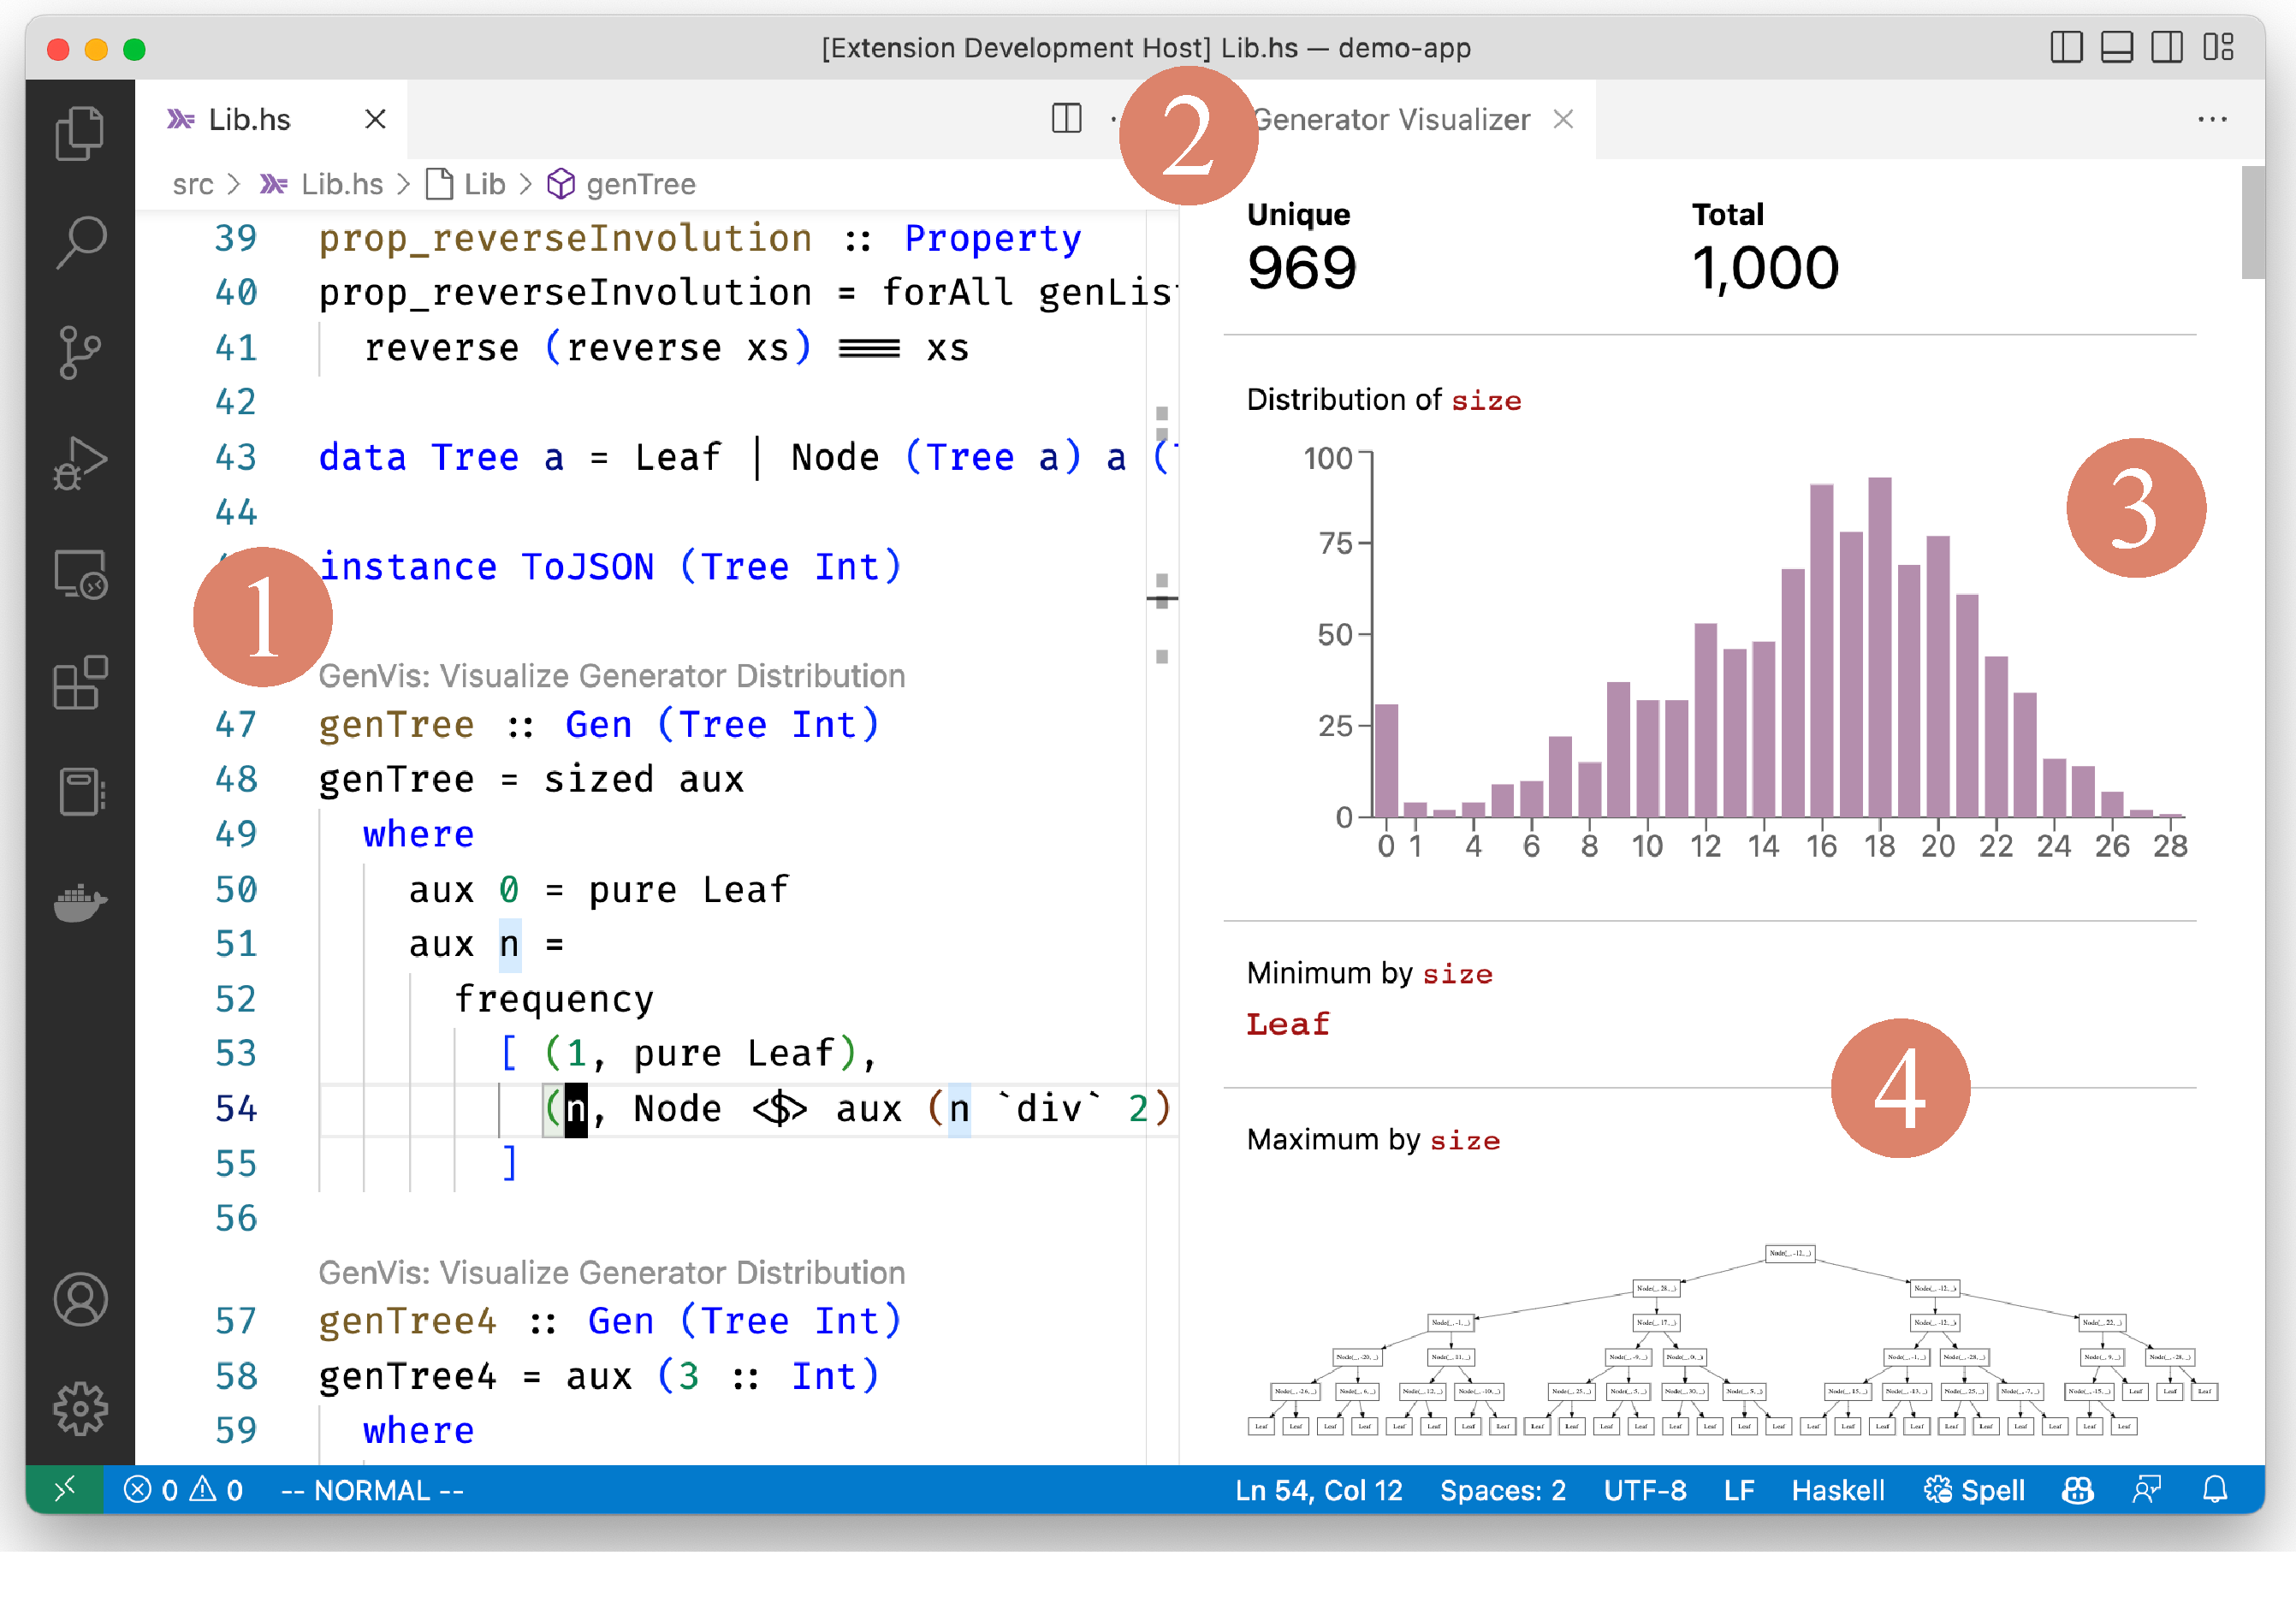
\includegraphics[width=0.6\textwidth]{assets/gen-vis.pdf}
  \caption{A mockup of our tool. (1) A {\em code lens} that the developer clicks
  to start the visualization. (2) High-level statistics about the generated values. (3)
  Charts displaying various data features. (4) Example values, rendered as
  graphs.}\label{fig:gen-vis}
\end{wrapfigure}

To help developers answer this question, we propose to build a tool that gives
developers comprehensive visualizations of their generators' distributions from
directly within their code editor. The tool will address the challenges with
visualizing generator distributions using a novel combination of tried-and-true
features can support the task of understanding the quality of input data
distributions. This includes (1) live, realtime displays of generated values;
(2) the ability to drill-down from aggregate displays to individual values; (3)
extensibility with lightweight hooks for customizing aggregate data displays and
previews of individual points; (4) live feedback on what code is covered by the
generated inputs.

Our tool starts by sampling a developer's generator and obtaining a set of
values to visualize. To get around the problem of arbitrarily structured data,
the system extracts and plots relevant {\em features} of a given datatype, that
will be extracted using functions in the surrounding programming environment and
validated by the user. In the case of the \lstinline{log} type above, we would
consider simple functions like \lstinline{length}, field accessors like
\lstinline{head}, \lstinline{id}, and \lstinline{payload}, filters like
\lstinline{is_empty}, and even aggregators
like \lstinline{maxBy} and \lstinline{avgBy}. Then the tool will then use
lightweight type-based program synthesis to compose and combine these functions
to get features. It may choose to show the \lstinline{length} of a log, but also
the \lstinline{maxBy (fun l -> length l.payload)} (the maximum payload length),
and even pairs of features like these (which could be viewed as a two
dimensional feature).  If there are features that the user notices should be
extracted, but that the system cannot come up with itself (e.g.,
\lstinline{ids_unique}) the user can write it themselves and add it to the
interface.

With the features extracted, the tool will then select various charts and
graphs to visualize the data, depending on its type. We are not yet certain
exactly which charts will be most helpful, but we will start with things like
histograms for discrete numerical data, pie charts for categorical data, scatter
plots for two dimensional numerical data, etc.  Of course, developers would
struggle to grok dozens of charts representing their data's features, so
we will also have a way for users to specify which visualizations are
interesting (and which to hide). We will base these interactions based on the
literature around visualization recommendation, specifically
Voyager~\cite{wongsuphasawat_voyager_2016, wongsuphasawat_voyager_2017}. This
interaction might be very quick (maybe a few seconds to find a single
representative chart) or slow and careful (many minutes spent curating a
dashboard of results to help with tuning), depending on how much time and energy
the developer has to put into their generator.

Another important aspect of understanding a generator's distribution is looking
at example values. We will therefore also present the user with views into some
of the generated values, which they can use to spot-check the generated data. As
we have mentioned, the shape and scale of these inputs may be
problematic---showing the user simple print-outs of the examples will not be
good enough. Thus, we propose potential ways of visualizing examples that may
become part of our tool. For inputs that are of a reasonable size, but where the
data {\em shape} is hard to see from text, we can give developers views of their
data structures as DOT graphs~\cite{ellson_graphviz_2002}; such graphs could be
generated via meta-programming and rendered for the user. When the input {\em size} is
the main barrier to understandability, we can take a more programmatic approach:
provide the user with the values represented as JSON objects, and give them
ways to manipulate those objects {\em in situ}.\hg{Did I use that right?}
This may involve exploring the data via mouse interactions (e.g., clicking to
expand or collapse sections) or even via a REPL with commands for filtering and
drilling into the structure.

As the project evolves, and once ``Bringing Fuzzing into Focus'' from
\sectionref{sec:fuzzing} is complete, we even plan to provide users with
visualizations of code coverage feedback.\hg{This feels weak here, let's see how
the end of the section ends up looking}

\amh{The visualization skeptic in me wonders if it will be possible come up with
generalizable DOT-based visualizations that work out of the box for most data
types. I would expect most visualizations to become unreadable once the number
of nodes in the data structures surpasses 10. We need to make a stronger case
that our automated features (including proposed visualizations types of filters)
will regularly work on the kinds of complexity of the data people will generate,
or otherwise shift to a goal of supporting developers in rapid definition of
their own filters and visualizations.}
\hg{Any better?}
\amh{Not really. I would prefer if the text directly
addressed the fact that generated inputs often have many
nodes for which conventional visualizations might not scale,
and propose some kind of solution (I am not sure the DOT
graphs would scale well). I think the JSON visualization
sounds the most promising, in conjunction with the ability
to use a REPL (I think I would leave out jq because it feels
like it would require many developers to learn another tool)
and the ability to write custom filters for viewing
individual data instances.}
\hg{For what it's worth, DOT graphs were my choice because it's what I actually
wanted to see as a user. If you're generating any kind of tree structures, the
shapes are really important, and one way or another that requires a visual
representation.  I'm hesitant to cut that completely...}

\todo{nice ending}

\todo{Evaluation plan}
All of these features will be made available to developers from within their
editor as a VSCode extension, and they will update live as the programmer edits
their generator and adds new functions that are candidates for extracting base
features. We will evaluate our tool in a small user study (around 15
participants), hoping to learn which features of the tool are most useful, and
how the design may be refined into a tool that real developers can use.
\amh{Probably instead of mentioning the
usability study here, we should factor this out into an
``evaluation plan'' that covers all of the tools in this
section.}

\SUBSECTION{Tuning Data Distributions}{sec:tuning}{1}{3}
\bcp{Why is this a Validation (as opposed to Generation) topic?  Also:
Do we want to front-load the topics with earlier start times, in their
respective sections.  (I'm just looking at the work plan table...)}
\hg{It's going to be a graphical approach to tuning based on GenVis, so it
wouldn't make much sense pulled out of context}

The tool proposed in the previous section will give developers unprecedented
visibility into their generator distributions, but what should they do if the
distribution is not the right one? Tuning generators is a challenging task~\cn{}
that would be much easier with the support of tools.

We propose extending the above visualization tool to include {\em bidirectional
interactions}: the developer will be able to select parts of the visualization
that seem wrong and edit them, causing changes to flow back into their editor as
modifications to the generator. These interactions include things like (1)
selecting points in a scatter plot to filter out; (2) dragging a bar on a bar
chart up or down, to indicate that a certain feature value should be more or
less represented; or (3) manipulating the sections of a pie chart to indicate
a better categorical distribution.

Some of these interactions can be implemented via {\em filtering}. Generators
already support operations that filter their outputs via predicates, so this is
a natural choice. If the user selects a range of values, as in interaction (1),
we can simply ask the generator to discard any values that do not fall in that
range.  However, filtering generators this way can be problematic: if the filter
is too broad, the generator will slow down significantly as it wastes time
generating inputs that it will have to discard.  We can protect users by
reporting a {\em discard rate} and warning them when that rate reaches a certain
threshold, but a more robust to altering the generator would be better.

Luckily, we may be able to both alleviate concerns around discard rates and
implement more interactions with the help of reflective generators (introduced
in \sectionref{sec:gen}). Recall that reflective generators can operate in
reverse, reflecting on the generator choices that produce a particular value. 
This means that if the user expresses a desire like ``category X should be
better represented'' (maybe by dragging a bar or a pie slice as in interactions
(2) or (3)), reflective generators can determine which choices often result in
values of that category and raise the weights on those choices. And this mode of
interaction can just as easily be applied to de-prioritize certain choices,
meaning that in some situations re-weighting with reflective generators can
obviate the need for expensive filters.

Ultimately we see this project and the previous one as a comprehensive toolkit
for generator customization. The understanding and tuning generators is too
often a cryptic process that users are inclined to avoid, to the detriment of
their testing success. With interactive tools, developers will be far more
likely to build useful generators that they can understand, and that they can
customize as they see fit.

\SUBSECTION{Turning Counterexamples into Regression Tests}{sec:counter}{3}{4}

\amh{Add references to Titus' slow fixes project,
CodeScoop, Emerson's work on visual extract-method
refactorings, and drag-n-drop refactoring, and test case
generation (e.g., RANDOOP).}

After a developer has identified a failure in their
property-based tests, they often wish to turn that failure
into a regression test, to ensure that later changes to the
code will not reintroduce the failure. One pain point
experienced by informants in our interview study was that it
required considerable work to transform a failure that was
already detected by their PBT tools into a regression test,
despite the fact that much of the work involved in doing so
felt mechanical.

We plan to develop usable tooling for transforming failed
PBT tests into single regression tests. What is important to
note about this project is that creation of regression tests
is \emph{mostly}, but not entirely mechanical. In reality,
the creation of regression tests will likely require
judicious incorporation of the developer's input at key
decision points. This is particularly the case for
specifying acceptance criteria. For instance, consider a
property that checks that a list insertion function never
produces an empty list. In the event of a failure, a
developer may want to produce a regression test checking the
exactness of the result for the failed input (i.e., checking
on a particular concrete list that should have been produced
by the insertion) rather than simply checking that the
output list is non-empty. The act of writing regression
tests involve several such choices, including\ldots{} \amh{I
ran out of time here.}

\amh{Refer to Hila's work.} \amh{Discuss with Harry to
figure out if we have something novel to contribute here.
Perhaps it would involve novel technologies around
shrinkers.}
\hg{This seems doable, as long as we think it's interesting... It strikes me as
a great engineering problem, but I'm not sure what the research angle is}
\amh{To create a test case, you need to unpack a property
into an input and an output, rather than just a property. Do
you want to test the property explicitly, or test for
exactness of the output? You need to remember that it is
failing case until after the bug is fixed\ldots{} once you
have the updated fixed function, then the output can be
plugged into expect test.}

\SUBSECTION{More Tests with Less Work}{sec:more}{3}{4}

\hg{This section needs honing; right now it's just what I wrote in my thesis
proposal, and it's too high-level} \amh{Is this a user
interface project devoted to figuring out ways of invoking
and keeping tabs on long-running tests during solo
programming? Or is it a project around proposing better
software engineering process that gives the right amount of
time to long-running PBT tests?}
\hg{Good question. I kind of naively hoped it was a UI project that both helped
users invoke and keep tabs of tests in the background AND pushed them towards
software engineering processes that gave PBTs appropriate space to operate. But
now that I think about it that seems like a lot at once. Honestly I think the
cultural shift in SE (potentially backed by some large-scale software tools) is
the more impactful angle, but I don't know if we can argue that we know how to /
want to do that}

The pilot study suggests that one area that new developer tooling may be
needed is in managing the interplay between PBT and continuous integration (CI)
systems. Recall that developers we spoke with pointed out frustration with the
fact that PBT is both nondeterministic and long-running. This combination left
them unsure of exactly where and when to test their properties: testing
properties locally slowed down their workflow, but testing them in CI
occasionally led them to find bugs at inconvenient times.

It is likely that PBT tools could play a role in improving this state of
affairs. For example, one could take inspiration from some theorem
provers~\cite{berghofer2004random} and create a system in which properties are
checked locally but in the background, as the programmer works on other things.
This avoids waiting time while potentially being less frustrating than running
in CI, since bugs would likely be found while the programmer still had the code
``paged in.'' Alternatively, one might design a PBT system with CI in mind,
providing automated features for deferring property failure notifications until
a specified time or turning failing properties into unit tests that can be saved
for future testing.

If the full-scale study indicates that this would be a useful line of work, we
will refine these ideas via user-centered design. Rather than build a system and
hope users like it, we will build minimal prototypes and iterate on the design
by observing testers using it. Ultimately we hope this will guide us to a tool
that will meaningfully improve the experience of PBT.

\SECTION{Education}{Advancing Testing in the Broader Culture \pagebudget{1}}{sec:ed}
\bcp{Needs some polishing and reintegration of the moved sections.}

\hg{This isn't actually written, this is just starter stuff from my thesis
proposal}\bcp{We need to do some actual, serious thinking about this.}

The pilot study also reminded us that PBT builds on concepts that are not
always comfortable for developers, and we expect that we will learn more about
the specifics of that discomfort in the large-scale study.  Prior work has
explored ways to close this knowledge
gap~\cite{wrenn2021using,nelson2021automated}, but we expect there are further
education challenges that are worth exploring.

I hope to work with the course staff of CIS 1210 to incorporate PBT into the
curriculum. The ideal scenario would be to add a PBT thread throughout the
course, giving students the tools to specify and test their code as they go.  I
plan to follow the lead of others who have done similar things before (e.g., the
PL folks at Brown University) to give students the best chance at incorporating
PBT into their tool-set.

There are a few important challenges that need to be considered in order for
this to work out.  The curriculum is already quite full, so adding PBT likely
means removing something else. I will need to work with the professors currently
teaching the course to find room, but I expect that this process will be fairly
difficult. It is also possible that adding PBT will actually make parts of the
course {\em easier}, especially for students with some knowledge of logic and/or
less well-developed unit testing instincts. Honestly I think this is a good
thing, as it gives students more ways to succeed and it may re-enforce the value
of PBT, but some may find this problematic.

\SUBSECTION{When to Specify It!}{sec:whento}{3}{4}
%
\bcp{The research content here (as described) is pretty minimal.
  Maybe this belongs in the education section instead?}
\hg{I think no. It'd take a bit of explaining elsewhere that I don't really want
to do, but more importantly I think it works as a real literature review /
survey / knowlege gathering exercise.  Let me know what you think of the
additions below; if you don't like it, we can just move the whole thing to edu
and fix the broken references}
%
PBT is often described as a kind of lightweight formal method, and one
might therefore imagine that a central challenge of using PBT would be
coming up with the
right specifications. Indeed, our pilot study concluded just that. But at
Jane Street we actually heard very little about the challenge of coming up with
properties; instead, most participants described applying PBT in scenarios when
properties were already available or quite easy to imagine. This suggests that,
while PBT educators should certainly spend some time teaching developers how to
write specifications for arbitrary programs, they should spend even more energy
helping developers quickly recognize situations where PBT is a particularly
natural fit because properties are obvious!

The study with Jane Street provides a solid start to a comprehensive list of
high-leverage use-cases for PBT. We have already identified seven software
patterns where properties are relatively straightforward to find and PBT is an
obvious choice for testing:
\begin{enumerate}[noitemsep]
\item Code that is already (semi-)formally specified.
\item Functions that round trip.
\item Pure data structures.
\item Modules with invariants.
\item Related versions of the same code.
\item Programs that may fail catastrophically.
\item Stateful APIs with well-understood contracts.
\end{enumerate}
These patterns are already quite broad in their scope, and include many
scenarios that real software developers regularly find themselves in, but they
are likely not exhaustive. Thus, we will continue to gather examples of
high-leverage use-cases: we will survey research papers and experience reports,
examine open-source software projects, and leverage our connections with various
PBT communities (QuickCheck/Haskell, Hypothesis/Python, Quickcheck/OCaml, etc.)
to ensure that we have a comprehensive understanding of the best uses for PBT.

Then,
we will compile a survey paper
(with an accompanying talk)
entitled {\em When to Specify It!} in homage to
John Hughes's {\em How to Specify It!}~\cite{HowToSpecifyIt}, a lovely
tutorial on the many different kinds of properties that one can write
for a given piece
of code. Clearly it is important to ask {\em How}, but our developer interviews
suggest that it may be even more important to have a clear sense of {\em When}
to use PBT. Our paper on {\em When to Specify It!} will combine examples from developer
interviews with ones from our our years of experience studying and applying PBT
into the definitive guide for the most impactful opportunities to apply PBT.

\SUBSECTION{Interactive Property Specification}{sec:interactive}{2}{3}

\bcp{General comment for this section: It all seems good, but it is a bit vague
and high level---I feel like technical readers will want a bit more meat.  Could
we spice it up with a concrete example?} \amh{Agreed, I think a concrete
example would be \emph{great} here. Maybe there is an example we can bring in
from the QuickSpec paper~\cite{claessen2010quickspec}}

\amh{Examples of complex properties that might not be
straightforward to implement. Algebraic properties of
libraries.  Reversing a list twice comes up with the same
list.  Properties of regular expressions. Maybe this would
be best as an educational tool. For instance, helping
students figure out how to test their code. Helping people
modularize their existing systems (suggestions to remove
depenedencies on Swing so that it is more testable, etc.).}

Preliminary findings from the Jane Street study suggest that developers sometimes have
difficulty imagining which properties to test, even when they believe their
software would benefit from property-based testing. One area we are interested
in exploring is how programmers can work with their PBT tools to decide on a set
of significant properties to test.  Prior research demonstrates that automated
tools can extract specifications of a program's
behavior~\cite{ammons2002mining,le2018deep,claessen2010quickspec}. We are
interested in the non-trivial research problem of integrating such techniques
into usable developer tools. We see the research as addressing several
challenges:

\textit{Generated properties should be \underline{important}}. Any non-trivial
program can be characterized by an overwhelmingly large number of properties,
many of which describe only incidental aspects of the program's behavior that do
not need to be tested. How can tools produce those properties that developers
would want to have tested? We believe that this is a problem that can be best
solved with a mixed-initiative approach~\cite{allen1999mixed}, where properties
are determined by judiciously incorporating both developer input and automated
techniques.

Developer could guide a specification mining tool to extracting relevant
properties through input mechanisms such as (1) identifying regions of code that
are likely to lead to an adverse behavior such as an exception or a logical
error; (2) providing unit test cases that test a special case of a generalized
property; and (3) indicating aspects of interest on input and output data during
exploration in a debugging REPL.

\textit{Generated properties should be \underline{readable}}. While prior research~\cite{claessen2010quickspec}
has shown promise for automatically generating specifications of program
behavior, we expect that users of PBT systems would benefit from having
properties generated in the language of their property-based testing tools.
Furthermore, there are some variants about systems that may be so complex that
they require significant comprehension time for users (i.e., those involving a
large number of clauses). In such cases, a tool may way to generate simpler
variants of properties first, and allow developers to refine them on their own.

\textit{Tools should help developers \underline{revise} properties}. If a generated
property is too relaxed, the tool should request that developer provides a
counterexample that should trigger a failure, and then regenerate the property.
If a generated property is too strict, a tool should allow a programmer to mark
a counterexample that was generated by the PBT tool as spurious, i.e., not
indicating an actual failure of the program. In each of these cases, the
property generator may have generate multiple properties for a developer to
review, each of which may satisfy the refinements that a developer has provided.

\textit{Plan of work}: We will iteratively design and develop developer tools as
an extension to the VSCode editor. In our first iterations, we will generate
candidate properties using QuickSpec~\cite{claessen2010quickspec}, a tool that
builds on Haskell's QuickCheck library to synthesize a series of plausible
properties about a given function. Future iterations will include tools like
\todo{cite other quickspec follow-on}~\cite{smith_discovering_2017}.
The interactions described above will be
designed and tested first for simple programs, and then on successively more
complex programs from our benchmark set. PI Head has extensive experience
designing and developing developer tools involving program
analysis~\cite{head2018interactive,head2019managing} and program
synthesis~\cite{head2017writing} components, and extending the VSCode
environment~\cite{head2020composing}.

\SUBSECTION{PBT in the Undergrad Curriculum}{sec:1210}{2}{4}
\bcp{Write me.  (Move stuff from upstairs?)}

\immediate\closeout\workplanfile
\SIMPLESECTION{Plan of Work \pagebudget{.7}}{sec:plan-of-work}

% \begin{figure}[ht]
%   \centering
%   \vspace*{-1in}
%   \hspace*{-.4in}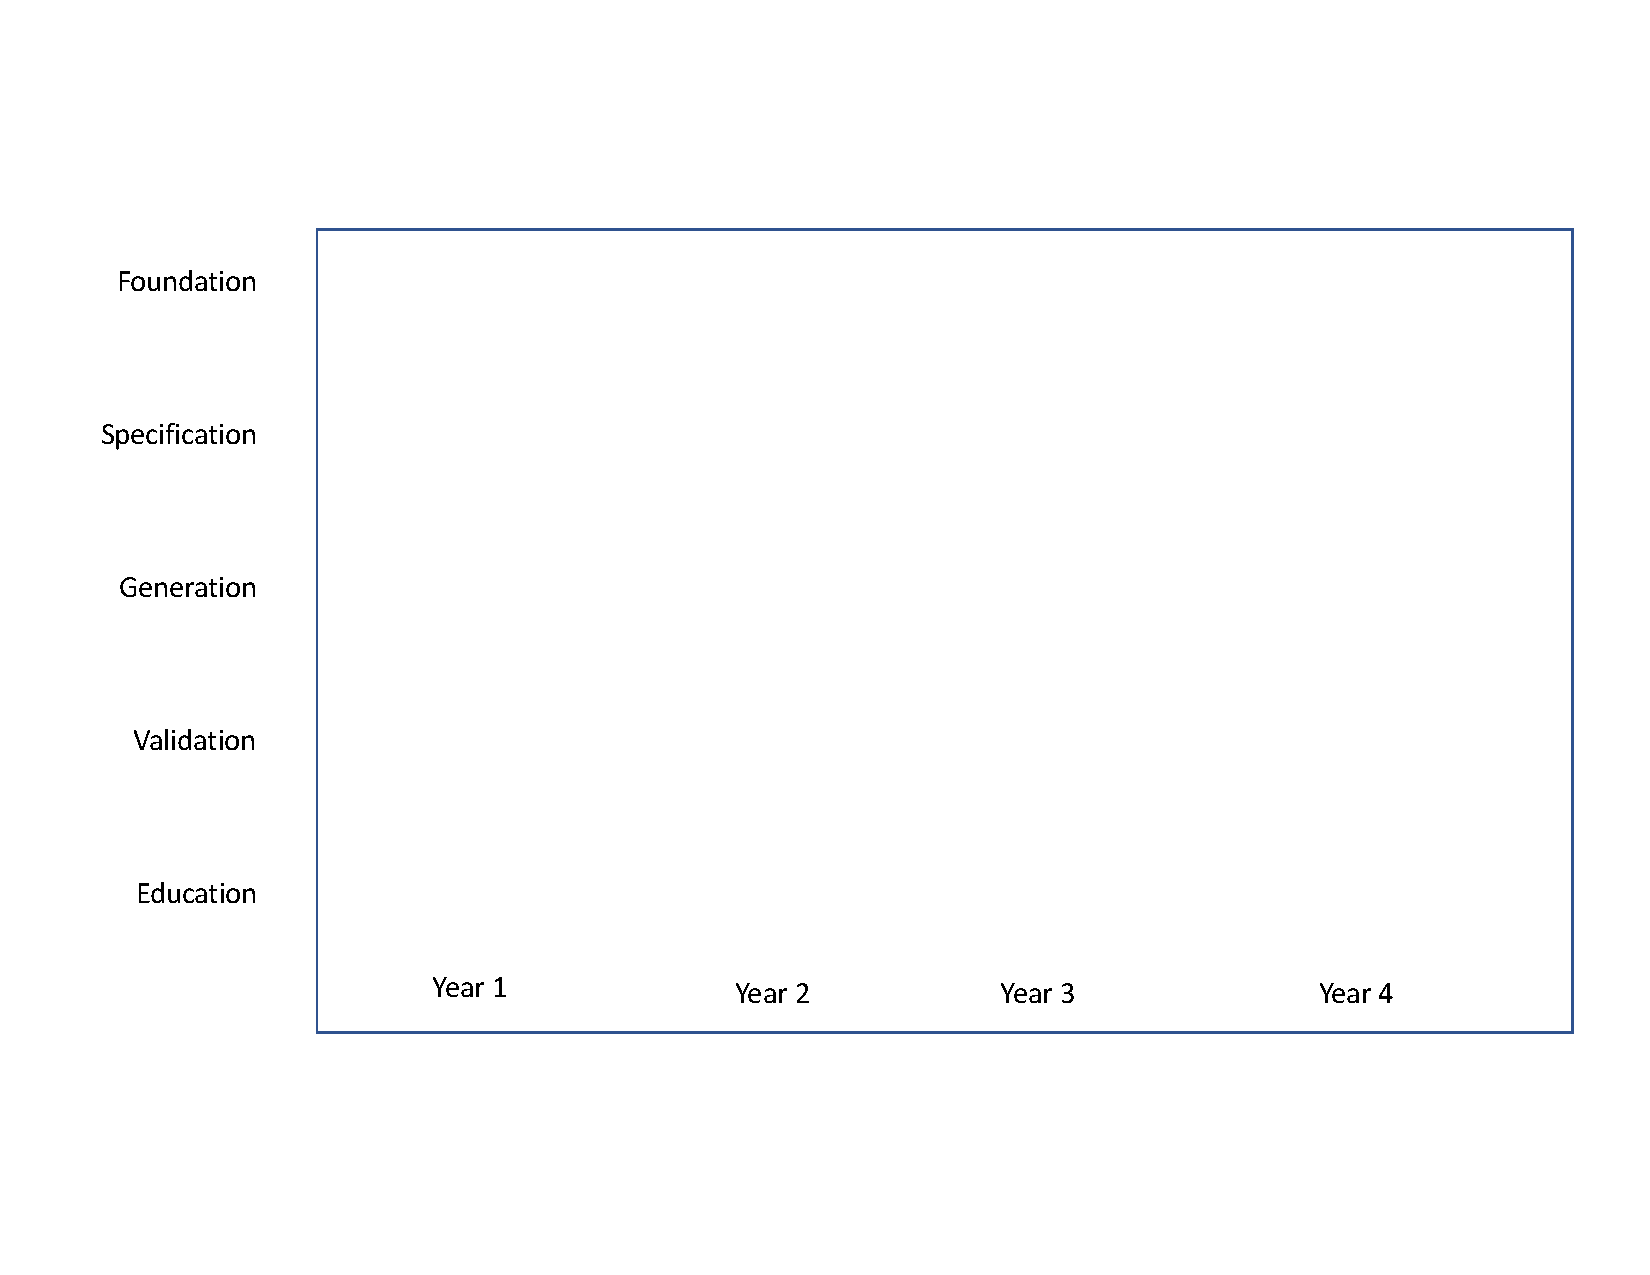
\includegraphics[width=1.1\textwidth]{assets/workplan.pdf}
%   \vspace*{-1.3in}
%   \caption{Plan of work.}\label{fig:workplan}
% \end{figure}

% \todo{Flesh out the chart in PPT; maybe eventually re-draw it in some
%   nicer form.}

\begin{figure}[ht]
  \centering
\begin{ganttchart}[
      expand chart=\textwidth,
      y unit chart=.4cm,
      %   vgrid
    ]{1}{4}
% \gantttitle{Ongoing}{1}
  \gantttitle{Year 1}{1}
  \gantttitle{Year 2}{1}
  \gantttitle{Year 3}{1}
  \gantttitle{Year 4}{1}
  % https://www.nsf.gov/pubs/policydocs/pappg22_1/pappg_2.jsp#IIB

\documentclass{NSF}

\graphicspath{{figures/}}

\usepackage{xcolor}
\definecolor{nord-night1}{HTML}{2e3440}
\definecolor{nord-night2}{HTML}{3b4252}
\definecolor{nord-night3}{HTML}{434c5e}
\definecolor{nord-night4}{HTML}{4c566a}
\definecolor{nord-snow1}{HTML}{d8dee9}
\definecolor{nord-snow2}{HTML}{e5e9f0}
\definecolor{nord-snow3}{HTML}{eceff4}
\definecolor{nord-frost1}{HTML}{8fbcbb}
\definecolor{nord-frost2}{HTML}{88c0d0}
\definecolor{nord-frost3}{HTML}{81a1c1}
\definecolor{nord-frost4}{HTML}{5579a5}
\definecolor{nord-red}{HTML}{b14853}
\definecolor{nord-orange}{HTML}{c76d52}
\definecolor{nord-yellow}{HTML}{ebcb8b}
\definecolor{nord-green}{HTML}{69894d}
\definecolor{nord-purple}{HTML}{815679}

\usepackage{listings}
\lstset{
  keepspaces=true,
  mathescape=true,
  frame=none,
  xleftmargin=10pt,
  stepnumber=1,
  belowcaptionskip=\bigskipamount,
  captionpos=b,
  % language=haskell,
  breaklines=true,
  tabsize=2,
  emphstyle={\bf},
  commentstyle=\it\color{cb-blue},
  stringstyle=\mdseries\ttfamily,
  showspaces=false,
  keywordstyle=\bfseries\ttfamily,
  deletekeywords={split},
  columns=flexible,
  basicstyle=\ttfamily,
  showstringspaces=false,
  morecomment=[l]--,
  moredelim=**[is][\color{nord-green}]{@}{@},
  moredelim=**[is][\color{nord-frost4}]{~}{~},
  moredelim=**[is][\color{nord-orange}]{£}{£},
  literate={cP}{{$\mathcal{P}$}}1
  {cG}{{$\mathcal{G}$}}1
  {cGhat}{{$\overline{\mathcal{G}}$}}1
  {cC}{{$\mathcal{R}$}}1
  {cL}{{$\mathcal{L}$}}1
  {fmap}{{$\fmap$}}3
  {[[}{{$\llbracket$}}1 % chktex 9
  {]]}{{$\rrbracket$}}1 % chktex 9
  % {->}{{$\rightarrow$}}2
  % {return}{{$\return$}}6
  % {pick}{{$\pick$}}4
  % {void}{{$\void$}}4
  % {do}{{$\textbf{do}$}}2
  % {>>=}{{$\bind$}}2
  % {<-}{{$\leftarrow$}}2
  % {\\}{{$\lambda$}}1
  % {==>}{{$\implies$}}3
  % {=>}{{$\Rightarrow$}}2
  % {<|>}{{$\langle | \rangle$}}2
}

\newcommand{\citet}[1]{\cite{#1}\todo{fixme}}
\newcommand{\citeauthor}[1]{\cite{#1}\todo{fixme}}

% Macros pilfered from HATRA submission
\definecolor{dkred}{rgb}{0.7,0,0}
\definecolor{dkpurple}{HTML}{4e02eb}
\definecolor{dkgreen}{HTML}{006329}
\definecolor{teal}{HTML}{007982}
\definecolor{string}{HTML}{02782d}
\definecolor{Fuchsia}{HTML}{8C368C}
\definecolor{quoteblue}{HTML}{2264b4}

\newif\ifdraft\drafttrue{}
\newcommand{\comm}[3]{\ifdraft\textcolor{#1}{[#2: #3]}\fi}
\newcommand{\cn}{\ifdraft{\color{blue} [CITE]}\fi}
\newcommand{\bcp}[1]{\comm{dkpurple}{BCP}{#1}}
\newcommand{\hg}[1]{\comm{dkred}{HG}{#1}}
\newcommand{\harry}[1]{\hg{#1}}
\newcommand{\jwc}[1]{\comm{dkgreen}{JC}{#1}}
\newcommand{\amh}[1]{\comm{teal}{AH}{#1}}
\newcommand{\comment}[1]{{\em #1}}
\newcommand{\todo}[1]{{\color{nord-red} TODO: #1}}
\newcommand{\pagebudget}[1]{(#1 pages)}

\newif\iflater\laterfalse

\usepackage{enumitem}

\begin{document}

\title{Property-Based Testing in Practice}
% \title{Property-Based Testing for the Working Programmer}
% \tableofcontents % TODO Remove?
%  BCP - was not working for me, so I followed the instruction to
%  remove :-)
\newpage

% A. Cover Sheet
% A number of the boxes contained on the Cover Sheet are
% electronically pre-filled as part of the FastLane login process
% Complete the rest of your info there

% B. Project Summary
\newsection{B}
\section*{Project Summary}

\todo{``Overview'' needed?}
\subsubsection*{Overview}
Property-based testing (PBT) is an advanced software engineering
methodology where users write executable formal specifications of system
components
and an automated test harness checks these specifications against
many automatically generated inputs.  The bug-finding power of PBT
arises its ability both to work with rich specifications and
to exercise a wide range of system behaviors---both
expected and unexpected---with minimal user guidance.
%
From its roots in the Haskell QuickCheck library, PBT has become
the testing method of choice across much of the functional programming
community; it has also begun to make inroads into industrial practice
at companies such as Quviq, Galois, Stripe, and
Amazon. \forreaders{Any other big companies?  Notable open-source
  projects?}
%
The goal of this proposal is to accelerate this transition
by addressing key challenges in
present-day PBT tools.

What are these challenges?
A need-finding study of PBT at Jane
Street, a Wall Street firm with a focus on software
technology as a competitive advantage, found developers enthusiastic
about its {\em usefulness} but
sometimes frustrated with its {\em usability}.
%
Indeed, the study identified usability as an issue in both major aspects
of PBT methods---{\em specification} of properties and {\em
  generation} of random inputs. Moreover, it revealed challenges
around another aspect of PBT that has so far received less attention from
researchers: how programmers can {\em validate} the
effectiveness of testing.

% At the level of {\em specification}, developers wished for better
% support for expressing common requirements such as ``this
% high-performance implementation of a service must behave exactly the
% same as that reference model'' and for articulating properties of
% poorly modularized code.
% %
% Concerning the other main component of PBT, the {\em generation} of
% random test cases, \todo{...}
% %
% Developers also need better {\em validation} tools for checking
% that their testing is actually effective.\todo{blah}
% %
% Finally, better {\em education} of potential PBT users is critically
% required.

% \amh{How about the following framing? In this project, we define a practice of
% usable property-based testing, and conduct foundational research in PL and HCI
% to bring about this practice. We define usable property based-testing as having
% two main components. First, providing visibility into what can be extremely
% complex test outcomes. Second, supporting the efficient expression of
% tests.\ldots{} And then we can jump into talking about the challenges that we
% plan to solve in specification, generation, validation, and education.}.
% %
% At the level of {\em specification}, developers wished for better
% support for expressing common requirements such as ``this
% high-performance implementation of a service must behave exactly the
% same as that reference model'' and for articulating properties of
% poorly modularized code.
% %
% Concerning the other main component of PBT, the {\em generation} of
% random test cases, \todo{...}
% %
% Developers also need better {\em validation} tools for checking
% that their testing is actually effective.\todo{blah}
% %
% Finally, better {\em education} of potential PBT users is critically
% required.

%  and ``shrinking'' of failing
% tests to minimal counterexamples,

To make PBT more usable, two largely disjoint
research areas must be
brought to bear.  PBT itself is grounded in domain-specific languages
and formal methods---traditional topics in the field of Programming Languages.
Usability, on the other hand, is the domain of Human-Computer Interaction.
%
This four-year project will combine insights, methods, and tools from
PL and HCI to advance the usability of PBT along all three of its
axes---specification, generation, and validation\iflater\todo{We may
  need to reorder these, depending on what happens with the global
  structure.}\fi---and bring it to a
broad community of software developers.

\smallskip

\noindent{\bf Keywords:} Programming languages; human-computer
interaction; property-based testing; usability.

\subsubsection*{Intellectual Merit}
The project will advance knowledge along four interconnected axes.
%
First, it will establish a firm {\bf\em foundation} for HCI-informed
research on PBT, supplementing past and ongoing user studies with
broader surveys of PBT across the software industry and real-time
observations of developers interacting with PBT.
%
Second, it will offer developers more usable {\bf\em specification} tools,
including a language for stating temporal properties over internal
program states and automation for model-based testing of
modular abstractions.
%
Third, it will explore a novel abstraction for random input {\bf\em
  generation} that enables a range of use cases---generating inputs
satisfying validity conditions, mutating inputs to explore the space
of similar inputs, and manually or automatically tuning a random
generator's distribution based on examples or code coverage.
%
And fourth, it will develop new interactive tools for rapid {\bf\em
  validation} of the effectiveness of testing, for helping programmers pin
down the causes of failures, and for visualizing generated data
distributions to support comprehension and tuning.

%  (1) deploy tools from HCI to better
% understand the challenges to wider adoption of PBT, (2) combine PL and
% HCI methods to build solutions, and (3) develop educational materials
% to make PBT concepts and tools accessible to a broad community of
% university students and industrial developers.

\subsubsection*{Broader Impacts}
A fifth thread of activity, coordinated with the rest and integral to the
project's aims, will be advance {\bf\em education} in PBT in both universities and industry. We will
develop materials for teaching industry programmers how to identify
high-leverage situations for using PBT, curricula for teaching mature
and powerful PBT practices to undergraduate students, and tooling to help
PBT beginners write their first properties.
%
A general-audience article on PBT for CACM will also help broaden the
reach of PBT.

Work on the project will include and elevate undergraduate
researchers, including some from diverse backgrounds that will be
funded through a new NSF-REU. These undergraduates will work
closely with the two PIs and four Ph.D.{} students in an interconnected and supportive
research environment.

The ultimate goal, through education, publications, and open-source
tools, is to make property-based testing a standard tool on every
software developer's testing toolbelt.  Better testing, in turn, will
lead to software systems of every sort that are less expensive, more
robust, and more reliable.


% The statement on broader impacts should describe the potential of the proposed activity to benefit society and contribute to the achievement of specific, desired societal outcomes.


% C. Table of Contents
% A Table of Contents is automatically generated for the proposal by FastLane

% D. Project Description
\newpage\newsection{D}
\section{Project Description \pagebudget{.5}}

\comment{Meta comment: I think a lot of the technical content here can come from my thesis proposal. It has all of the technical projects other than the benchmarking project (which BCP should be able to write about — or maybe ask for Jessica’s help?) and it also has the background and related work. It may be useful to go to the individual papers for some deeper details, but I’d be surprised.}

\todo{Harry proposal page 4 and 6.5-8}

\todo{
[MODEL AFTER THESIS INTRO / CONCLUSION]
\begin{itemize}
   \item High level: Advance the theory and practice of PBT, making it more valuable to a wider range of software engineers
   \item PBT is great
\begin{itemize}
      \item For people who like formal methods, it’s a way to write a formal spec and check it without doing full verification
      \item Even for people who don’t, it’s been extremely effective finding bugs in practice
         \item Cite…
      \item (?) And people really like it (maybe pull quotes from preliminary study)
\end{itemize}
   \item But there is still room for PBT to grow (maybe stats, feel free to refine this argument more)
   \item We want to advance the theory and practice of PBT so it is more valuable to SEs
\end{itemize}
}

\subsection{Background and Related Work \pagebudget{1.5}}

\subsubsectionstar{PIs' Prior Qualifications}

\subsection{Extending the Foundation \pagebudget{3}}

\todo{
\begin{itemize}
   \item Story
\begin{itemize}
      \item The research community has identified that random generation (and in particular, the valid generation problem)[b] causes problems for testers
      \item This shows up in prior work, and also in realistic examples (e.g., the fuzzing community really cares about this!)
      \item We’ve already done some work to explore new abstractions for random generation (free generators) and we have more that we want to try (reflective generators)
      \item In addition, the PBT community is missing tools to empirically evaluate generation strategies
      \item And the PBT literature is also woefully disconnected from the fuzzing literature, where they have their own partial solutions to this problem
\end{itemize}
   \item Prior Work - Free generators [CHAPTER 1[c] OF THESIS PROPOSAL is a
   source, but it's way too long -- we need to write a compact precis of the
   crucial points]
   (perhaps also some other prior things)
   \item Planned Work - Reflective generators [CHAPTER 2 OF THESIS PROPOSAL]   (needs new work on evaluation; maybe rests on benchmarking infrastructure; validity-preserving mutation scheme needs to be evaluated by real implementation and measurement)
   \item Planned Work - Empirical Evaluation Playground [JESSICA OR BENJAMIN WRITE] (can ultimately be used for Benchmarking; in the short term, it’s a playground for individual PBT efforts to see how they are doing)
   \item Speculative Work - Add PBT incrementally to a fuzzing system [CHAPTER 3 OF THESIS PROPOSAL](follows directly from the free and reflective generators work)
\end{itemize}
}

\subsection{Finding out what working programmers need \pagebudget{3}}

\todo{
\begin{itemize}
   \item Story
\begin{itemize}
      \item The projects above follow the lead of prior work, solving problems that have already been identified, but we have no reason to believe that those problems are exhaustive
      \item Indeed, there may be high-leverage opportunities to improve PBT that have nothing to do with the valid generation problem
      \item We’re in the process of uncovering “unknown unknowns” by talking to PBT users about their experiences - we’ve already done a preliminary study, and we plan on talking to Jane Street developers for a full-scale study
      \item We’re not sure what we should do after that, but the preliminary study gave us some ideas
\begin{itemize}
         \item We can obviously keep talking to users (via surveys or observations)
         \item We also identified that there are likely workflow improvements that could help PBT fit into a developer’s environment better (and user-centered design opportunities there)
         \item We may even find interesting PBT opportunities at Jane Street that will give us a hands-on opportunity to solve problems that real developers are actively dealing with
\end{itemize}
\end{itemize}
   \item Prior Work - Pilot study [CHAPTER 4 OF THESIS PROPOSAL / HATRA]
   \item Planned Work - Jane Street Study [CHAPTER 4 OF THESIS PROPOSAL / HATRA]
\end{itemize}
}


Part 1 of the ``unknown unknowns''.
Jane Street study, preliminary study, observations, surveys.

In this aim, we plan to set course for research in PBT, both broadly and for the
future directions of our group. We will conduct a series of formative studies,
each addressing one of three main goals:

\subsubsectionstar{Understanding Challenges to Using PBT Tools}

The first step is to conduct qualitative interviews to understand the challenges
that programmers face when using PBT tools.

Here I will elaborate on the design of the Jane Street study.

\subsubsectionstar{Characterizing the Potential Reach for PBT Tools}

We will conduct a survey with the purpose of understanding the impact that
improved PBT tools could have in industry, if major usability issues were
addressed. We see this survey as crucial in understanding the amount of
resources that should be devoted to PBT research. Furthermore, this
questionnaire will help shed light into which of the usability challenges from
the interview study, if addressed, are most likely to impact a broad set of
current and prospective users of PBT tools.

\subsubsectionstar{Understanding the Structure of PBT Tasks in Detail}

The next step is to more deeply characterize the obstacles faced with specific
tools and tasks through close observation. We anticipate conducting observations
of participants formulating properties and creating generators, as we expect
that close observation of developers performing these tasks will yield yet
additional detail about ways that developers are supported and not supported by
the tools they use today to a level of depth we will not achieve with the
interviews.

\subsection{Exploiting the Foundations to Build Powerful, Interactive PBT Tools \pagebudget{3}}

Upon the advanced technical foundation from Aim 1 and the refined understanding
of programmers' needs from Aim 2, our final aim (Aim 3) will focus on the
development of programmer-facing tools that allow them to leverage properties in
testing their code more efficiently and effectively.

While the specific focus of our tool design and research efforts will be
continually refined on the basis of what we learn from Aim 2, below we detail
several directions that we expect to lead to the design of tools that are both
innovative within the research community, as well as potentially impactful,
drawing on the lessons learned from the preliminary need-finding research we
have done to date as well as our own intuitions, and as critical users and
engaged members of the communities for these tools.

\todo{Discuss:

\begin{itemize}

% \item Some of the tools we propose in this section may depend on a technical
% background we do not have on this team. For instance, property generation.
% Should we be keeping the scope of the proposed work to those where we as a team
% have expertise in the backend technologies? After discussing with BCP, we need
% not limit ourselves to areas where we are at present the leading experts. Let's
% draft the descriptions, see the ones we are excited about, wave away some
% of the details that we have not yet educated ourselves, and go from there.

\item We should ask Jane Street for a letter of support indicating their
willingness to collaborate on the need-finding activities.

\end{itemize}
}

\subsubsectionstar{Interactive property specification}

Developers in the preliminary interview study indicated that while they knew their software would benefit from property-based testing, sometimes they had difficulty imagining which properties to test. One area that could benefit from innovation in PBT tools is in designing tools that help programmers imagine properties in situations like these.

To date, research has shown the potential for automated tools to extract invariants describing a program's behavior\cite{ammons2002mining,le2018deep,claessen2010quickspec}. However, the integration of such tools into developer workflows is non-trivial. We posit that a usable tool that can help with imagining properties would need the following features:

\textit{Readable code generation}. While prior techniques have succeeded in generating invariants, we expect that users of PBT systems would benefit from having properties generated in the language of their property-based testing tools. Furthermore, there are some variants about systems that may be so complex that they require significant comprehension time for users (i.e., those involving a large number of clauses). In such cases, a tool may way to generate simpler variants of properties first, and allow developers to refine them on their own.

\textit{Generating important properties}. Non-trivial programs can be described by an overwhelmingly large number of properties, many of which describe only incidental aspects of the program's behavior that do not need to be tested. How can tools produce those properties that developers would want to have tested? We believe that this is a problem that can be best solved with a mixed-initiative approach~\cite{allen1999mixed}---that is, judiciously incorporating both developer input and automation. Developer could guide a specification mining tool to extracting relevant properties through input mechanisms such as (1) identifying regions of code that are likely to lead to an adverse behavior such as an exception or a logical error; (2) providing unit test cases that test a special case of a generalized property; and (3) indicating aspects of interest on input and output data during exploration in a debugging REPL.

\textit{Property refinement}. Tools could help a developer refine generated properties. If a generated property is too relaxed, the tool could request that developer provides a counterexample that should trigger a failure, and then regenerate the property. If a generated property is too strict, a tool could allow a programmer to mark a counterexample that was generated by the PBT tool as spurious, i.e., not indicating an actual failure of the program. In each of these cases, the property generator may have generate multiple properties for a developer to review, each of which may satisfy the refinements that a developer has provided.

\textit{Plan of work}: Incorporating known, widely-used specification mining tools such as QuickSpec~\cite{claessen2010quickspec}\ldots{}

% One challenge identified by software developers we have spoken with is that it can be difficult to come up with a property to test with property-based testing tools. Perhaps tools could help programmers come up with, and express, properties that they wish to be tested. To design such tools, we will adapt techniques from the specification mining literature to generate candidate properties (e.g.,~) and interfaces that help programmers select from, and refine, generated properties.
% 
% A first step will be to generate candidate properties. These will be generated using specification mining techniques. Specifications will need to be mapped from an abstract representation of the property to an expression of that property in the programming language, such as Hypothesis' property specification language. A major challenge is that a specification mining technique will produce many spurious properties which do not describe aspects of the program that the programmer wishes to test. Affordances will be added to the programming environment to allow a program to select subsets of code that manipulate properties of interest; and to generalize from behaviors that are implied by individual unit tests, or observations made during debugging, to greatly limit the space of generated properties.
% 
% A second step will be to assist in the refinement of properties. In some cases, generated properties will be too broad; for instance, . if the testing tools yield a counterexample, the counterexample may be an indicator that a property is insufficiently strict, rather than an indication that the program is incorrect. @Andrew, continue from here\ldots{}
% 
% Motivation: Informants struggled to figure out what to test. informants had an intuitive idea of what “right” and “wrong” was. Perhaps they could have been helped with a tool that refined that expectation into something that was formal.
% 
% Plan of work: A first step in this process might be a tool that refines a wrong specification that has some counterexamples into a clean, correct specification. When a counterexample is encountered, you can fix the program if it represents a bug, or you will have to refine a property if the property was not written correctly.
% Alternatively, a greenfield specification maker might depend on a machine learning backend. We need to know more about how this works. Perhaps speak to Mayur about unit test generation. The tool design would focus on coming up with usable property specifications, and potential some user input (e.g., pointing to parts of programs that should be involved in property creation). Could specifications be provided as natural language? QuickSpec works okay for Haskell using static analysis to determine invariants. We would need someone with ML or program synthesis background to work on this project.
% 
% Example: For a serialization / deserialization pair of functions, testing that the serialized deserialized string is the same version as the original string; the refinement is to exclude Unicode strings, which do not have to be supported by serialization functions.

\subsubsectionstar{Visualizing and tuning data distributions}

% (this topic is what Joe is most excited about)

% For visualizing data distributions...

Plan of work: easily computable summary statistics; as well as user-defined metrics for understanding what you care the most about from the distribution. Seeing what the “average” data structure is that is getting generated. For multimodal data, what are the different modes of data. The set of data types to be handled in PBT are: algebraic data types, lists, trees (this would also cover programs). Joe thinks we already have good visualizations for numbers, booleans, and strings; it is compositional data types that we lack good visualizations for. People need to (1) see representative examples (2) understand spread (3) indicate areas of the space that should not be explored.

% For tuning data distributions...

Plan of work: indicating areas of the distribution that should not be generated.

Example: writing a generator of programs (for instance, to test out a compiler). You want lots of different programs that make sense in different ways. You want large ones, small ones, ones that use variables in coherent ways, ones that don’t overuse certain constructs, ones that use a variety of different language features. You want the generated programs to be representative of those that people might write. You also want some weird programs to catch the edge cases, but you don’t want all weird programs. (How big, how deep, how wide of programs?). Also, for trees, one might want to specify heights and breadths of the tree.

\subsubsectionstar{Debugging support for understanding counterexamples}

Once a PBT tool generates a counterexample of where a property fails, a programmer will need to understand what in an input caused the program to fail. This task can be rather challenging because generated inputs can be complex, deep data structures \todo{Do we have a reference that implies the complexity of generated counterexamples?}. Methods for making it clearer why a counterexample fails could be to generate additional inputs that are very close to the counterexample that are actually correct, to run the program up to the point where the traces of the programs begin to diverge, and then to drop a programmer into a debugging environment where they can query the state of the program and step through the remainder of the execution. PI Head has prior work designing debugging tools that help programmers understand trace divergences in an educational setting~\cite{suzuki2017tracediff}.

\subsubsectionstar{Reconciling generator API design with imperative language idioms}

Motivation: How do you design a generator DSL in an imperative language? A generator uses higher-level functions in a way that might be confusing to people who used Python.  (e.g., passing a generator of numbers to a generator of lists to get randomized lists of numbers). Is there a way of designing APIs for generators that can make the composition of these types of generators easier to reason about and express for some programmers?

(Joe says the DSLs are well-designed, but the code is hard to debug. How do you write a generator that works really well, that has a good data distribution and finds bugs? See below.)

Plan of work. Not sure. This might require some discussions with more uses of Hypothesis-like libraries.

Next steps—get examples of sloppily-expressed PBtests in Python and then think through how they would be written more clearly.

\subsubsectionstar{Integration with continuous integration workflows}

\todo{Section 6.2 of Harry's thesis proposal.}

\subsubsectionstar{Tailoring PBT for financial systems}

I am not sure what should go here. I am a bit wary of focusing specifically on developing tools for financial systems if the focus of this grant proposal is to make PBT tools more broadly useful.

\subsection{Education \pagebudget{1}}

\subsection{Plan of Work \pagebudget{.5}}

\subsection{Broader Impacts \pagebudget{.5}}
The Project Description must contain, as a separate section within the narrative, a section labeled ``Broader
Impacts of the Proposed Work". This section should provide a discussion of the broader impacts of the proposed
activities. Broader impacts may be accomplished through the research itself, through the activities that are
directly related to specific research projects, or through activities that are supported by, but are complementary to
the project. NSF values the advancement of scientific knowledge and activities that contribute to the
achievement of societally relevant outcomes. Such outcomes include, but are not limited to: full
participation of women, persons with disabilities, and underrepresented minorities in science, technology, engineering, and
mathematics (STEM); improved STEM education and educator development at any level; increased public
scientific literacy and public engagement with science and technology; improved well-being of individuals in
society; development of a diverse,globally competitive STEM workforce; increased partnerships between
academia, industry, and others; improved national security; increased economic competitiveness of the United
States; and enhanced infrastructure for research and education.

\subsection{Results from Prior NSF Support \pagebudget{.5}}
If any PI or co-PI identified on the project has received NSF funding (including any current
funding) in the past five years, in formation on the award(s) is required,
irrespective of whether the support was directly related to the proposal or not.
In cases where the PI or co-PI has received more than one award (excluding amendments),
they need only report on the one award most closely related to the proposal. Funding includes not just salary
support, but any funding awarded by NSF. The following information must be provided:\\

\noindent
\emph{\underline{Name of PI}}: NSF-Program (Award Number) ``Title of the Project'' (\$AMOUNT, PERIOD OF SUPPORT).
{\bf Publications:} List of publications resulting from the NSF award. A complete bibliographic citation for each
publication must be provided either in this section or in the References Cited section of the proposal); if
none, state: ``No publications were produced under this award.'' {\bf Research Products:} evidence of research products
and their availability, including, but not limited to: data, publications, samples, physical collections, software,
and models, as described in any Data Management Plan.

% \subsubsection{Proposed Study}
% The Project Description should provide a clear statement of the work to be undertaken and must include:
% objectives for the period of the proposed work and expected significance; relation to longer-term goals of the PI's
% project; and relation to the present state of knowledge in the field, to work in progress by the PI under other
% support and to work in progress elsewhere.
%
% The Project Description should outline the general plan of work, including the broad design of activities to be
% undertaken, and, where appropriate, provide a clear description of experimental methods and procedures.
% Proposers should address what they want to do, why they want to do it, how they plan to do it, how they will
% know if they succeed, and what benefits could accrue if the project is successful. The project activities may be
% based on previously established and/or innovative methods and approaches, but in either case must be well
% justified. These issues apply to both the technical aspects of the proposal and the way in which the project may
% make broader contributions.

\subsection{More stuff to not forget :-)}

Unfunded collaborations: Any substantial collaboration with individuals not included in the budget should be described in the Facilities, Equipment and Other Resources section of the proposal (see Chapter II.C.2.i) and documented in a letter of collaboration from each collaborator. Such letters should be provided in the supplementary documentation section of FastLane or Research.gov and follow the format instructions specified in Chapter II.C.2.j. Collaborative activities that are identified in the budget should follow the instructions in Chapter II.D.3.

Remember to not use any URLs in the project description!  (They are
encouraged in the references.)


% E. References Cited
\newpage\newsection{E}
\renewcommand\refname{References Cited}
\bibliography{andrew,harry,bcp}
% I prefer to use the IEEE bibliography style.
% That's  NOT required by the NSF guidelines.
% Feel Free to use whatever style you prefer
% \bibliographystyle{ACM-Reference-Format}
\bibliographystyle{IEEEtran}

% F. Biographical Sketch(es)
\newpage\newsection{F}
See here for advice on how to write these:
\url{https://www.nsf.gov/bfa/dias/policy/disclosures_table/june2021.pdf}

% G. Budget Justification
\newpage\newsection{G}
\iflater
\section*{Budget Justification}

\todo{GPG: Budgets for all projects must include funding for one or
  more designated project representatives (PI/co-PI/senior researcher
  or NSF-approved replacement) to attend each annual PI meeting during
  the proposed lifetime of the award.}

\todo{GPG: a portion of the budget for each Core Programs, Large
  Projects proposal may be used to engage relevant Broadening
  Participation in Computing (BPC) expertise to help plan, organize,
  coordinate and execute BPC activities.}

\todolater{Make sure to account for PhD months accurately---note when
  people start.}

\hg{Any chance we want to budget for a new machine for someone (e.g., one or
more of the potential other PhD students)? Or is that priced in?}
\bcp{Good catch -- yes, we want to budget for new machines for all.
  Possibly also a server, for running lots of tests faster...}

\todo{REPL students (see comments here)}
% And attached is the budget sheet from PEFS. The TLDR yearly costs are….

% Direct Student Costs
% ================
% Travel - $400 per student per year
% Housing - $2500 per student per year
% Stipend - $6000 per student per year

% Indirect Student Costs
% =================
% Admin - $32,500 per year (10k for lead admin, 10k distributed across PLClub+ leaders, with Penn’s 62.5% overhead stacked on top)

% Let me know if you have any questions. If you want to contribute to indirect student costs, I’m not totally sure what the right amount is — but it seems we’re currently charging about $4,000 per student per year in admin costs.

\discuss{Should we be asking for budget for a compute server or AWS or
  any other Cloud Computing service (e.g., NSF itself has one)), for
  running heavy testing workloads??  If not, we should say so.  The
  benchmarking project, for example, could use this!}

% No more than 3 pages!!!
\subsection*{A. Senior Personnel}
\noindent{\bf A1.} Includes two PIs at 18\% CY.
\subsection*{B. Other Personnel}
\noindent{\bf B3.} Includes stipend for one graduate student for each calendar year of the project.

\todo{Webinar: Staff support is normal.  Needs to justified not only
  in the body of the proposal but also carefully called out in the
  budget justification.}

\subsection*{C. Fringe Benefits}
Fringe benefits are calculated at a rate of X\% for faculty, Y\% for graduate students.
\subsection*{E. Travel}
1) all travel (both domestic and foreign) must now be justified.
2) temporary dependent care costs above and beyond regular dependent care that directly result from travel to conferences are allowable costs provided that the conditions established in 2 CFR § 200.474 are met.
\subsection*{G. Other Direct Costs}
1) Includes coverage on costs of computing devices
2) The charging of computing devices as a direct cost is allowable for devices that are essential and allocable, but not solely dedicated, to the performance of the NSF award
\noindent{\bf G5.} Includes tuition for graduate students participating in the program.
\subsection*{H. Indirect Costs}
Overhead at a rate of X\% is charged on all direct salaries and wages, applicable fringe benefits, materials and supplies, services, travel and subawards up to the first \$X of each subaward. Excluded are equipment and the portion of each subaward in excess of \$X.
\fi


%  H. Current and Pending Support
\newpage\newsection{H}
\section{Current \& Pending Support}
\begin{tabular}{ll}
\textbf{Investigator:} 			& \\
\textbf{Project Title:}			& Put your Proposal title here\\
\textbf{Project Location:}		& \\
\textbf{Source of Support:} 	& NSF\\
\textbf{Total Award Amount:} 	& \\
\textbf{Total Award Period:}	& \\
\textbf{Status:}				& Pending (this project) \\
\end{tabular}


% I. Facilities, Equipment and Other Resources
\newpage\newsection{I}
\section*{Facilities, Equipment, and Other Resources}

Penn's departmental computing facilities include a standard collection of
networking services, printers, fileservers, and compute servers.  No
specialized facilities or equipment will be needed to carry out the
proposed work.

\todo{Mention, here, any machines we've budgeted for in the budget
  section?}

\hg{Other things off the top of my head then: travel for speaking, meetings, and
conferences (lots), REPL funding (talking to Joey next week), desk setups for
the new students, a bit of money for hosting PBT-focused PLClub speakers? ---
I'm just guessing at stuff, just take the parts that make sense}

\discuss{
Document all three (four?) unfunded external collaborations.
  \begin{itemize}
  \item Any substantial collaboration with individuals not included in
  the budget should be described in the Facilities, Equipment and
  Other Resources section of the proposal (see Chapter II.D.2.g) and
  documented in a letter of collaboration from each collaborator. Such
  letters should be provided in the supplementary documentation
  section of Research.gov and follow the format instructions specified
  in Chapter II.D.2.i. 
  \item We also need to make sure that the appropriate sections of the
  project description mention the collaborations.
  \end{itemize}
}





% J. Special Information and Supplementary Documentation
\newpage\newsection{J}
\section*{Data Management Plan}

The project will produce four types of data.

\begin{enumerate}
\item Software artifacts,
including implementations, test cases, software revision histories, and
other items.  These will be distributed under an open-source
license.  They will be documented so as to allow others to understand,
use, and modify them.  (Both PIs have extensive records of
distributing artifacts in this way.)  Artifacts will be made available
to the public on Github and maintained for at least three years beyond
the end of the project lifecycle.

\item Technical papers and talks describing our experiences
and results.  These will be published in academic conferences and journals.
Drafts will be made available on Arxiv.

\item Educational materials aimed at undergraduates, masters students,
and professional developers, which will be made available on the
project's public website under an open-source license.

\item Raw data gathered during user studies, which will be kept
confidential and stored securely in accordance with IRB-approved best
practices.
\end{enumerate}

\iflater{%
\amh{Consider integrating the following, which Andrew wrote up for his NSF
CAREER to address more of the concerns the data management plan is asked to
address.}

\paragraph{Data from usability evaluations} As part of routine tool design and
evaluation activities, we will collect human subjects data in the form of questionnaire responses, interface usage
logs, and, during lab evaluations, screen recordings, audio recordings, and
researcher notes. Data will be collected from users in the following settings: (1)
in-lab usability studies; (2) interviews and observations with expert authors;
(3) instructor usage of the tools to augment instructional materials in CIS 545 and CIS 421; (4) student
use of augmented documents in the same classes; and (5) usage of the
tools in the wild.

All data from human subjects will be collected, stored, and analyzed in accordance
with institutional best practices following procedures that have undergone review by Penn's Institutional
Review Board. In all circumstances, users' express consent will be obtained
prior to collection and analysis of data. Data will be handled in a way that is sensitive
to the following considerations:

\emph{Confidentiality}. User confidentiality will be preserved by collecting
only those identifiers absolutely necessary to manage studies and conduct the required
analyses. Identifiers that need to be collected will be removed from the data when it
becomes possible to do so: for instance, audio recordings will be transcribed and then
deleted to remove the identifier of participants' voices, and identifiers (like
names and company affiliations) will be removed from transcripts. Participants will
be able to request that we delete or redact usability data should it contain information that is sensitive for them. Any transcription services that we use will have signed strict confidentiality agreements.

\emph{Security}. Human subjects data will be collected, stored, and analyzed on password-protected,
encrypted machines managed by research personnel who have undergone human subjects research
training. The data may also be stored on secured departmental servers and password-protected
shared folders hosted in university-approved cloud services.
We will retain data long enough that the Ph.D. student researcher can consult it throughout their entire program of study. Our plan is to retain study data for seven years following the project start date. After that time, the data will be deleted.
}
		% Data Management Plan (Required)
%\input{sections/postdoc} % Postdoctoral Researcher Mentoring Plan (if applicable)

\end{document}

\end{ganttchart}
  \caption{Plan of work.  \iflater\bcp{It's too big probably.  :-(  We can
      trim it a little by removing the main section headings.  After
      that, is it interesting enough to justify the space?  I guess we
    could alternatively include ``(Years X to Y)'' in subsection
    titles}\bcp{Can squeeze one line at the top by hacking a bit.}\fi}\label{fig:workplan}
\end{figure}

\todo{Write words}

\SIMPLESECTION{Broader Impacts \pagebudget{.5}}{sec:broader-impacts}
The Project Description must contain, as a separate section within the narrative, a section labeled ``Broader
Impacts of the Proposed Work". This section should provide a discussion of the broader impacts of the proposed
activities. Broader impacts may be accomplished through the research itself, through the activities that are
directly related to specific research projects, or through activities that are supported by, but are complementary to
the project. NSF values the advancement of scientific knowledge and activities that contribute to the
achievement of societally relevant outcomes. Such outcomes include, but are not limited to: full
participation of women, persons with disabilities, and underrepresented minorities in science, technology, engineering, and
mathematics (STEM); improved STEM education and educator development at any level; increased public
scientific literacy and public engagement with science and technology; improved well-being of individuals in
society; development of a diverse,globally competitive STEM workforce; increased partnerships between
academia, industry, and others; improved national security; increased economic competitiveness of the United
States; and enhanced infrastructure for research and education.

\bcp{Education is described in its own separate section.}

\SIMPLESECTION{Results from Prior NSF Support \pagebudget{.5}}{sec:prior}
If any PI or co-PI identified on the project has received NSF funding (including any current
funding) in the past five years, in formation on the award(s) is required,
irrespective of whether the support was directly related to the proposal or not.
In cases where the PI or co-PI has received more than one award (excluding amendments),
they need only report on the one award most closely related to the proposal. Funding includes not just salary
support, but any funding awarded by NSF. The following information must be provided:\\

\noindent
\emph{\underline{Name of PI}}: NSF-Program (Award Number) ``Title of the Project'' (\$AMOUNT, PERIOD OF SUPPORT).
{\bf Publications:} List of publications resulting from the NSF award. A complete bibliographic citation for each
publication must be provided either in this section or in the References Cited section of the proposal); if
none, state: ``No publications were produced under this award.'' {\bf Research Products:} evidence of research products
and their availability, including, but not limited to: data, publications, samples, physical collections, software,
and models, as described in any Data Management Plan.

% \SUBSECTION{Proposed Study}
% The Project Description should provide a clear statement of the work to be undertaken and must include:
% objectives for the period of the proposed work and expected significance; relation to longer-term goals of the PI's
% project; and relation to the present state of knowledge in the field, to work in progress by the PI under other
% support and to work in progress elsewhere.
%
% The Project Description should outline the general plan of work, including the broad design of activities to be
% undertaken, and, where appropriate, provide a clear description of experimental methods and procedures.
% Proposers should address what they want to do, why they want to do it, how they plan to do it, how they will
% know if they succeed, and what benefits could accrue if the project is successful. The project activities may be
% based on previously established and/or innovative methods and approaches, but in either case must be well
% justified. These issues apply to both the technical aspects of the proposal and the way in which the project may
% make broader contributions.

\iflater
\section*{More stuff to not forget :-)}

Unfunded collaborations: Any substantial collaboration with
individuals not included in the budget should be described in the
Facilities, Equipment and Other Resources section of the proposal (see
Chapter II.C.2.i) and documented in a letter of collaboration from
each collaborator. Such letters should be provided in the
supplementary documentation section of FastLane or Research.gov and
follow the format instructions specified in Chapter
II.C.2.j. Collaborative activities that are identified in the budget
should follow the instructions in Chapter II.D.3.  \bcp{Jane Street.
  And maybe we should ask John too?}

bpc.net - source materials for NSF BPC plans (they also vet plans).
  we should check that other universities are doing!

\fi
